\documentclass[11pt]{article}

\usepackage[UTF8,scheme=plain]{ctex}
\usepackage[margin=1in]{geometry}
\usepackage{amsmath}
\usepackage{booktabs}
\usepackage{float}
\usepackage{graphicx}
\usepackage{subcaption}
\usepackage[hidelinks]{hyperref}
\usepackage{pgfplots}
\pgfplotsset{compat=1.18}
\renewcommand{\tablename}{表}
\renewcommand{\figurename}{图}

\title{FQAHC 数值结果汇总：ED、DMRG 与光学响应}
\author{Partial Hall Crystal Project}
\date{\number\year 年 \number\month 月 \number\day 日}

\newcommand{\phitwopi}{\Phi_y/2\pi}
\newcommand{\qmid}{Q_{\mathrm{mid}}}

\begin{document}
\maketitle

\section{文档目的}

本文档汇总 ED 与 DMRG 的基准数值、正式计算参数、电荷泵浦、能谱、结构因子和
光学响应。能谱、静态结构因子与 response-Lanczos 光电导均由 ED 计算；
Lanczos 的作用是在 Hilbert 空间很大时不显式求出全部激发态。大型波函数和 DMRG
原始输出有意保存在 git 之外；本文档只收录汇总数值和体积较小的数据与图片。

\section{模型与几何}

DMRG 模块研究圆柱上的完整双带实空间模型。几何在 \(x\) 方向采用开放边界，
在 \(y\) 方向采用周期边界。对于下文使用的 \(L_y=6\) 圆柱，
\[
  N_s = L_x L_y, \qquad N_{\mathrm{uc}} = N_s/2 = 3L_x,
  \qquad N_p = N_{\mathrm{uc}}/3 = L_x .
\]
正式计算采用参数
\[
  t_1=1.0,\qquad t_3=0.2,\qquad V_1=1.0,\qquad V_2=V_3=0.0 .
\]

\section{圆柱 ED 与 DMRG 基准}

第一个小系统检验将 DMRG 与同一个圆柱 Hamiltonian 的精确对角化结果比较，
而不是与 torus Hamiltonian 比较。数据保存在 W003 的
\begin{center}
\small\path{dmrg/output_Lx4/energy_check.dat}.
\end{center}

\begin{table}[h]
\centering
\caption{零通量下 \(L_x=4,L_y=6,N_p=4\) 的圆柱基准。}
\begin{tabular}{llr}
\toprule
物理量 & 方法 & 能量 \\
\midrule
基态能量 & 圆柱 ED & \(-9.238777471721946\) \\
基态能量 & DMRG & \(-9.238777009200746\) \\
绝对差值 & \(|E_{\mathrm{DMRG}}-E_{\mathrm{ED}}|\) & \(4.6252120000644936\times 10^{-7}\) \\
\bottomrule
\end{tabular}
\end{table}

作为对照，此处跟踪的 \(4\times6,N_p=4\) 数据在 torus 边界下的 ED 结果为
\[
  E_{\mathrm{torus}} \simeq -9.31357589 .
\]
因此
\[
  E_{\mathrm{cyl}} - E_{\mathrm{torus}}
  \simeq 0.07479842 .
\]
这一差值来自边界条件：圆柱删去了跨越开放 \(x\) 边界的 hopping 和相互作用项，
并具有真实边缘。上面的 ED--DMRG 一致性验证了圆柱 MPO 以及符号和指标约定，
但并不意味着圆柱与 torus 的能谱相同。

\section{Lx=15 warm-start 谱流计算}

下述 \(L_x=15\) 谱流数据来自 warm-start 正式计算，不是上面
\(L_x=4\) 的 ED--DMRG 小系统基准。计算所用系统为
\[
  L_x=15,\quad L_y=6,\quad N_s=90,\quad N_{\mathrm{uc}}=45,\quad
  N_p=15,\quad \nu=N_p/N_{\mathrm{uc}}=1/3 .
\]

\begin{table}[h]
\centering
\small
\caption{\(L_x=15\) warm-start 谱流的正式 DMRG 设置。}
\begin{tabular}{p{0.28\linewidth}p{0.62\linewidth}}
\toprule
项目 & 数值或设置 \\
\midrule
计算目录 & \path{dmrg/flux_Lx15_pump_prod_20260710_170505} \\
几何 & 开放 \(x\)、周期 \(y\) 的完整双带实空间圆柱 \\
Hamiltonian 参数 & \(t_1=1.0,\ t_3=0.2,\ V_1=1.0,\ V_2=V_3=0.0\) \\
通量方向 & 圆柱 \(y\) 周期上的扭转 \(\Phi_y\) \\
Warm-start 流程 & 分段保存 checkpoint 的轨迹；分支细化从 \path{forward_pi12/checkpoints/state_017.jls} 开始 \\
绘图网格 & \path{forward_pi12}: \(\Delta\Phi=\pi/12\)；\path{branch_from_fwd17_pi24}: \(\Delta\Phi=\pi/24\)；\path{branch_from_fwd17_pi36}: 跳变附近 \(\Delta\Phi=\pi/36\) \\
随机种子 & \path{forward_pi12} 为 1234，\path{branch_from_fwd17_pi24} 为 1357，\path{branch_from_fwd17_pi36} 为 9753 \\
最大 bond dimension & \(200,400,800,1200,1600,2000\) \\
截断阈值 & \(10^{-9}\) \\
Sweep 控制 & \(\texttt{max\_sweeps}=40\), \(\texttt{retry\_sweeps}=40\), \(\texttt{max\_retries}=2\), \(\texttt{min\_sweeps}=4\), \(\texttt{stable\_sweeps}=3\) \\
收敛门槛 & \(\Delta E\le 10^{-6}\)，最大密度变化 \(\le 2\times10^{-5}\)，截断误差 \(\le 5\times10^{-8}\)，并设置 \(\texttt{REQUIRE\_CONVERGED=true}\) \\
线程目标 & W003 上每个节点使用 24 个 CPU core \\
绘图点状态 & 48/48 个绘图点均满足 \(\texttt{converged=true}\)；最差诊断值为 \(\Delta E=1.87403\times10^{-7}\)、密度变化 \(1.48122\times10^{-5}\)、截断误差 \(5.868\times10^{-9}\) \\
\bottomrule
\end{tabular}
\end{table}

\section{电荷泵浦观测量}

图中电荷定义为中心截面左侧的累积密度变化：
\[
  Q(x,\Phi_y)=\sum_{x'\le x,y}
  \left[\langle n_{x',y}\rangle_{\Phi_y}
  - \langle n_{x',y}\rangle_{\Phi_y=0}\right].
\]
绘制的量为 \(\qmid\)，其截面取在圆柱中心附近。由于总粒子数固定，
一直累积到右边缘所得的总电荷变化近似为零。

\section{通量插入结果}

图中直接使用下列文件中的原始 \(\texttt{cumulative\_mid}\) 列；文件位于
\begin{center}
\small\path{/home/public/shajy/partial_Hall_crystal/dmrg/flux_Lx15_pump_prod_20260710_170505}.
\end{center}
\begin{itemize}
  \item \path{forward_pi12/pumping.dat}
  \item \path{branch_from_fwd17_pi24/pumping.dat}
  \item \path{branch_from_fwd17_pi36/pumping.dat}
\end{itemize}
数据没有经过 sector 展开、分支重新标记，也没有手动加上 \(1/3\) 平移。

\begin{table}[h]
\centering
\caption{\(L_x=15\) warm-start 谱流数据中选取的原始数据点。}
\begin{tabular}{llrrr}
\toprule
\(\phitwopi\) & 数据序列 & 步数 & 原始 \(\qmid\) & 能量 \\
\midrule
0.000000 & \path{forward_pi12} & 0  & 0.000000000 & \(-35.0036151955\) \\
0.500000 & \path{forward_pi12} & 12 & 0.166481976 & \(-34.9065831468\) \\
0.750000 & \path{forward_pi12} & 18 & 0.254744645 & \(-34.8726423200\) \\
0.791667 & \path{forward_pi12} & 19 & 0.269989638 & \(-34.8696299183\) \\
0.805556 & \path{branch_from_fwd17_pi36} & 24 & 0.275054113 & \(-34.8686784085\) \\
0.819444 & \path{branch_from_fwd17_pi36} & 25 & -0.059271363 & \(-34.9843387311\) \\
1.000000 & \path{forward_pi12} & 24 & -0.000000131 & \(-35.0036151660\) \\
\bottomrule
\end{tabular}
\end{table}

\begin{figure}[h]
\centering
\begin{tikzpicture}
\begin{axis}[
    width=0.94\linewidth,
    height=0.52\linewidth,
    xmin=0, xmax=1,
    ymin=-0.09, ymax=0.35,
    xlabel={\(\phitwopi\)},
    ylabel={原始 \(\qmid\)},
    grid=both,
    legend style={at={(0.02,0.98)},anchor=north west,font=\small},
    legend cell align={left},
]
\addplot[forget plot,draw=none,fill=black!10] coordinates {
  (0.805556,-0.09) (0.819444,-0.09) (0.819444,0.35) (0.805556,0.35)
} \closedcycle;
\addplot[dashed,thick,gray!70!black] coordinates {(0,0) (1,0.333333333)};
\addlegendentry{\(\nu=1/3\) 参考线}
\addplot[blue,thick,mark=*] coordinates {
  (0.000000,0.000000000000)
  (0.041667,0.013653577203)
  (0.083333,0.027321412226)
  (0.125000,0.041013687529)
  (0.166667,0.054739402328)
  (0.208333,0.068506101876)
  (0.250000,0.082319845336)
  (0.291667,0.096185540981)
  (0.333333,0.110107556282)
  (0.375000,0.124090620428)
  (0.416667,0.138140885842)
  (0.458333,0.152267148419)
  (0.500000,0.166481976122)
  (0.541667,0.180802468817)
  (0.583333,0.195250318056)
  (0.625000,0.209850354519)
  (0.666667,0.224626783225)
  (0.708333,0.239594793140)
  (0.750000,0.254744645424)
  (0.791667,0.269989638488)
  (0.833333,-0.054694481836)
  (0.875000,-0.040987638755)
  (0.916667,-0.027309661164)
  (0.958333,-0.013650769530)
  (1.000000,-0.000000130997)
};
\addlegendentry{\(\Delta\Phi=\pi/12\)}
\addplot[red!70!black,thick,mark=square*] coordinates {
  (0.729167,0.247152214355)
  (0.750000,0.254748775556)
  (0.770833,0.262371248861)
  (0.791667,0.269995119594)
  (0.812500,-0.061561451232)
  (0.833333,-0.054694553046)
  (0.854167,-0.047836927420)
  (0.875000,-0.040987644795)
  (0.895833,-0.034145620002)
  (0.916667,-0.027309657901)
  (0.937500,-0.020478489426)
  (0.958333,-0.013650771527)
  (0.979167,-0.006825127140)
  (1.000000,-0.000000128455)
};
\addlegendentry{\(\Delta\Phi=\pi/24\)}
\addplot[green!50!black,thick,mark=triangle*] coordinates {
  (0.722222,0.244629032651)
  (0.736111,0.249681784414)
  (0.750000,0.254749923131)
  (0.763889,0.259830565970)
  (0.777778,0.264917559155)
  (0.791667,0.270000671593)
  (0.805556,0.275054113004)
  (0.819444,-0.059271363022)
  (0.833333,-0.054694553579)
};
\addlegendentry{\(\Delta\Phi=\pi/36\)}
\end{axis}
\end{tikzpicture}
\caption{\(L_x=15\) warm-start 谱流的原始电荷数据。灰色区域表示
\(\Delta\Phi=\pi/36\) 细化计算中观察到的最窄原始跳变窗口
\(0.805556 \le \phitwopi \le 0.819444\)。彩色数据点是未经修改的
\(\texttt{cumulative\_mid}\)；没有加入 \(1/3\) 的分支偏移，也没有展开 sector。}
\label{fig:charge-pump-raw}
\end{figure}

\section{原始分支跳变说明}

原始电荷在 \(\phitwopi=0.805556\) 处平滑增加至
\(\qmid\simeq0.275054\)，随后在 \(\phitwopi=0.819444\) 跳变至
\(\qmid\simeq-0.059271\)。跳变量接近 \(-1/3\)，但本文保留 DMRG 实际收敛到的
sector 中的原始数据。在开放边界和近简并基态流形下，这个原始不连续应被视为
可能的分支切换，而不是已经展开好的平滑泵浦曲线。若要确定 sector 归属，
还需要 MPS overlap、纠缠谱流或显式态跟踪流程等额外诊断。

\clearpage
\section{光电导：Kubo 求和与 response-Lanczos}
\label{sec:optical-conductivity}

本节记录旧版显式 sum-over-states 程序和修正后的 response-Lanczos 基准所采用的
线性光学响应约定。这里只讨论线性电导。在使用相同 Hamiltonian 和电流算符时，
两种数值方法计算的是同一个多体 resolvent；二者的区别在于计算方式，而不是物理量。
需要特别强调：这里的 exact sum-over-states 与 response-Lanczos 都属于 ED，
不是 DMRG 动力学响应。

\subsection{电磁场约定与算符}

对于沿 Cartesian \(x\) 方向的均匀矢势，定义
\begin{equation}
  H(A_x)=H(0)+A_xJ_x+\frac{A_x^2}{2}K_{xx}+O(A_x^3),
  \qquad
  J_x=\left.\frac{\partial H}{\partial A_x}\right|_{0},
  \qquad
  K_{xx}=\left.\frac{\partial^2H}{\partial A_x^2}\right|_{0}.
  \label{eq:optical-operators}
\end{equation}
修正后的有限 torus 实现统一从
\begin{equation}
  H_A(k)=H(k+A_x\hat{x})
  \label{eq:bloch-ax}
\end{equation}
构造 \(H(A_x)\)、\(J_x\) 和 \(K_{xx}\)。这里 \(A_x\) 是单位 Cartesian 长度上的
均匀矢势，而不是总 twist。对于 \(4\times6\) torus，\(\Phi_x=4A_x\)。
本文取 \(e=\hbar=1\)，并采用算符符号约定
\(J_x=\partial H/\partial A_x\)。

对于基态 \(\lvert g\rangle\)，引入
\begin{equation}
  Q=1-\lvert g\rangle\langle g\rvert,
  \qquad
  \lvert f\rangle=QJ_x\lvert g\rangle,
  \qquad
  z=\omega+i\eta,
  \label{eq:response-source}
\end{equation}
对于每个与源向量耦合的激发态，再定义
\begin{equation}
  \Delta_n=E_n-E_g,
  \qquad
  w_n=\left|\langle n\rvert J_x\lvert g\rangle\right|^2.
\end{equation}

\subsection{显式态求和的 Kubo 公式}

完全对角化给出有限系统的 resolvent
\begin{align}
  G(z)
  &=\langle f\rvert\left[z-(H-E_g)\right]^{-1}\lvert f\rangle
    =\sum_{n\ne g}\frac{w_n}{z-\Delta_n}, \\
  \chi(z)
  &=G(z)+G(-z)
    =\sum_{n\ne g}w_n
      \left(\frac{1}{z-\Delta_n}-\frac{1}{z+\Delta_n}\right), \\
  \chi_0
  &\equiv\chi(0)=2\operatorname{Re}G(0)
    =-2\sum_{n\ne g}\frac{w_n}{\Delta_n}.
  \label{eq:exact-resolvent}
\end{align}
旧 ED 脚本中实际使用的纵向响应表达式可以逐个本征态整理为
\begin{align}
 &\frac{w_n}{iz}
  \left(\frac{1}{z+\Delta_n}-\frac{1}{z-\Delta_n}\right)
  +\frac{2iw_n}{z\Delta_n} \\
 &\hspace{1.4cm}=\frac{iw_n}{z}
  \left[
    \frac{1}{z-\Delta_n}-\frac{1}{z+\Delta_n}
    +\frac{2}{\Delta_n}
  \right].
\end{align}
对 \(n\) 求和后，响应可写成
\begin{equation}
  \sigma_{xx}^{\mathrm{old}}(z)
  =\frac{2\pi i}{A_{\mathrm{old}}}
   \frac{\chi(z)-\chi_0}{z},
  \label{eq:old-kubo}
\end{equation}
它对应下文定义的 regular 有限频率电导，而不是包含独立计算的抗磁项的 total 响应。

\subsection{regular、Drude 与 total 电导}

采用有限 torus 的物理面积 \(A\)，定义
\begin{align}
  D_{xx}&=\langle g\rvert K_{xx}\lvert g\rangle+\chi_0, \\
  \sigma_{xx}^{\mathrm{Drude}}(z)
    &=\frac{2\pi i}{A}\frac{D_{xx}}{z}, \\
  \sigma_{xx}^{\mathrm{reg}}(z)
    &=\frac{2\pi i}{A}\frac{\chi(z)-\chi_0}{z}, \\
  \sigma_{xx}^{\mathrm{total}}(z)
    &=\sigma_{xx}^{\mathrm{Drude}}(z)
      +\sigma_{xx}^{\mathrm{reg}}(z)
      =\frac{2\pi i}{A}
       \frac{\langle K_{xx}\rangle+\chi(z)}{z}.
  \label{eq:conductivity-parts}
\end{align}
这些量都是复电导。为了明确每幅图中实部和虚部的来源，令 \(X=X'+iX''\)，并写成
\begin{equation}
  \sigma_X(z)=\frac{2\pi i}{A}\frac{X}{\omega+i\eta}.
\end{equation}
于是
\begin{align}
  \operatorname{Re}\sigma_X
   &=\frac{2\pi}{A}
     \frac{\eta X'-\omega X''}{\omega^2+\eta^2}, \\
  \operatorname{Im}\sigma_X
   &=\frac{2\pi}{A}
     \frac{\omega X'+\eta X''}{\omega^2+\eta^2}.
  \label{eq:real-imag-source}
\end{align}
三类电导对应的分子分别为
\begin{equation}
  X_{\mathrm{Drude}}=D_{xx},\qquad
  X_{\mathrm{reg}}=\chi(z)-\chi_0,\qquad
  X_{\mathrm{total}}=\langle K_{xx}\rangle+\chi(z).
\end{equation}

\begin{table}[h]
\centering
\small
\caption{各类纵向复电导的含义与来源。}
\begin{tabular}{p{0.20\linewidth}p{0.34\linewidth}p{0.34\linewidth}}
\toprule
物理量 & 实部 & 虚部 \\
\midrule
\(\sigma^{\mathrm{reg}}\) & 经 \(\eta\) 展宽的有限频率吸收谱 &
regular 响应的反应性/色散部分，是吸收谱的 Kramers--Kronig 伴随量 \\
\(\sigma^{\mathrm{Drude}}\) & 展宽后的零频 Drude 贡献；当
\(\eta\to0^+\) 时趋于 delta 函数贡献 & 反应性 Drude 极点，在远离零频时趋于
\(1/\omega\) \\
\(\sigma^{\mathrm{total}}\) & regular 与 Drude 实部之和 & regular 与 Drude
虚部之和 \\
\bottomrule
\end{tabular}
\end{table}

有限 torus 上的 \(D_{xx}\) 是所选有限尺寸 twist 与动量分支上的曲率组合。
单个固定 twist 上出现负值，不能直接解释为热力学极限中负的耗散 Drude weight；
要作这种判断，需要跟踪随 twist 变化的全局基态并进行尺寸外推。

基准数据文件保存了四幅修正后分量图所使用的 exact 和最终 Lanczos 数值：
\begin{table}[H]
\centering
\small
\caption{\texttt{optical\_response\_curves.dat} 各列的含义。}
\begin{tabular}{cl}
\toprule
列 & 保存的响应 \\
\midrule
2--3 & Exact \(\operatorname{Re/Im}\sigma^{\mathrm{total}}\) \\
4--5 & Lanczos \(\operatorname{Re/Im}\sigma^{\mathrm{total}}\) \\
6--7 & Exact \(\operatorname{Re/Im}\sigma^{\mathrm{reg}}\) \\
8--9 & Lanczos \(\operatorname{Re/Im}\sigma^{\mathrm{reg}}\) \\
\bottomrule
\end{tabular}
\end{table}

\subsection{完全对角化与 response-Lanczos}

exact 参考结果显式构造并完全对角化有限 \(m=2\) sector 中的 Hamiltonian，
随后使用保存的全部 \(\Delta_n\) 和 \(w_n\) 计算
Eq.~\eqref{eq:exact-resolvent}。它对这个有限 sector 和指定展宽是精确的，
但不代表热力学极限的精确结果。

Response-Lanczos 从 \(q_1=\lvert f\rangle/\lVert f\rVert\) 出发，并生成递推
\begin{equation}
  (H-E_g)q_j
  =\beta_{j-1}q_{j-1}+\alpha_jq_j+\beta_jq_{j+1}.
  \label{eq:response-lanczos-recurrence}
\end{equation}
若 \(T_M\) 是由此得到的三对角矩阵，则同一个 resolvent 可近似为
\begin{align}
  G_M(z)
  &=\lVert f\rVert^2 e_1^{\mathsf T}(zI-T_M)^{-1}e_1 \\
  &=\frac{\lVert f\rVert^2}
  {z-\alpha_1-\dfrac{\beta_1^2}
  {z-\alpha_2-\dfrac{\beta_2^2}{\ddots}}}.
  \label{eq:lanczos-continued-fraction}
\end{align}
因此，完全对角化的 sum-over-states 与 response-Lanczos 是计算同一个 Kubo
resolvent 的两种 ED 方法。前者显式求得相关激发本征态并逐态求和；后者从
\(QJ_x\lvert g\rangle\) 出发，在 Krylov 空间内计算 resolvent，因此无需求出或保存
全部激发态。response-Lanczos 不是 DMRG 响应算法，它是面向更大 ED sector 的方法。

\subsection{历史线性响应图片}

\paragraph{历史结果状态说明。}
下面的图片保留为早期线性响应计算记录，不能作为修正后算符的验证数据。
旧脚本实际使用的 \(x\) 方向速度为 \(v_1\)，Cartesian 组合当时被注释；
速度算符的构造还复用了可能加入相互作用的 Hamiltonian apply 路径；
归一化采用 \(L_1L_2\) 而不是 torus 的物理面积。另外，先折叠
\(d_x=\pm L_x/2\) 的 hopping 路径再求导会得到错误的 \(J_x\) 和 \(K_{xx}\)，
尽管 \(H(0)\) 及其能谱本身不受影响。

\begin{figure}[p]
\centering
\begin{subfigure}{0.48\linewidth}
  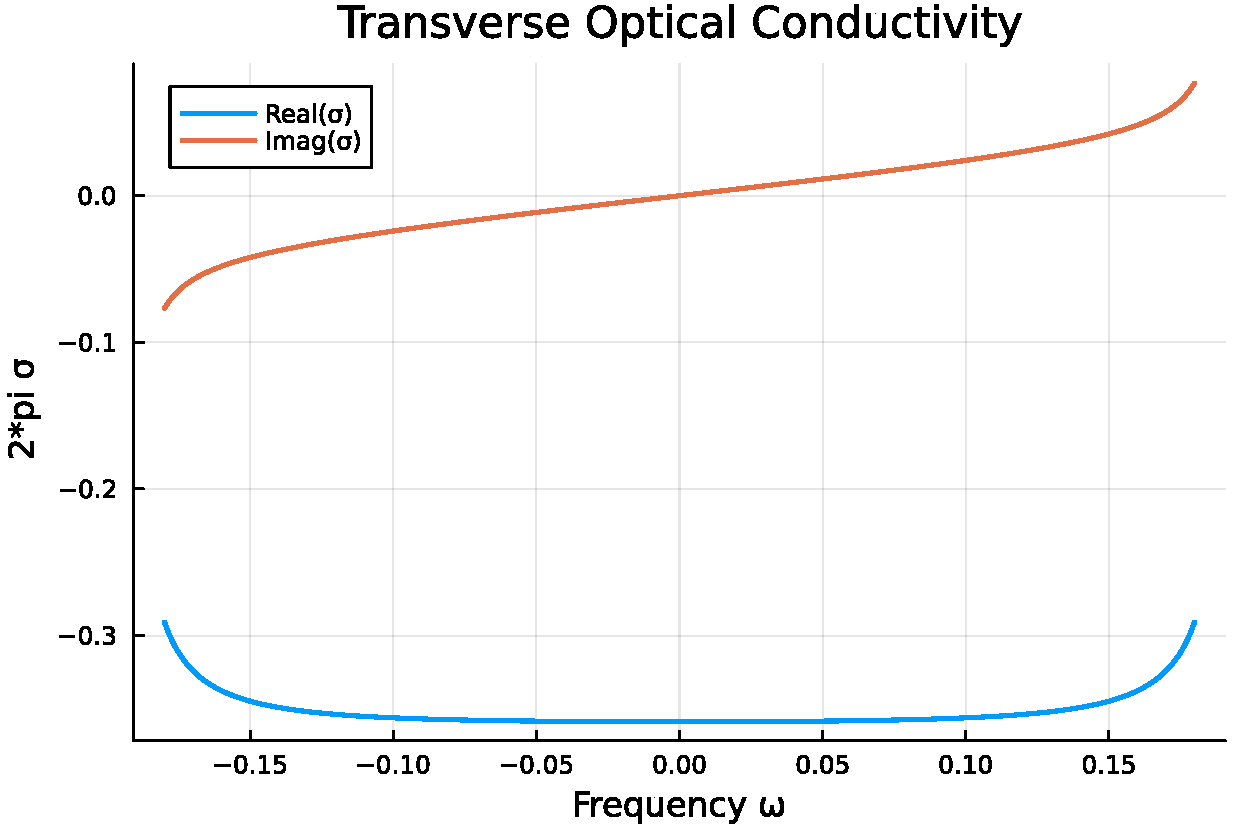
\includegraphics[width=\linewidth]{figures/optical_response/legacy_optical_conductivity.pdf}
  \caption{文件名中没有记录展宽参数的历史横向响应图。}
\end{subfigure}\hfill
\begin{subfigure}{0.48\linewidth}
  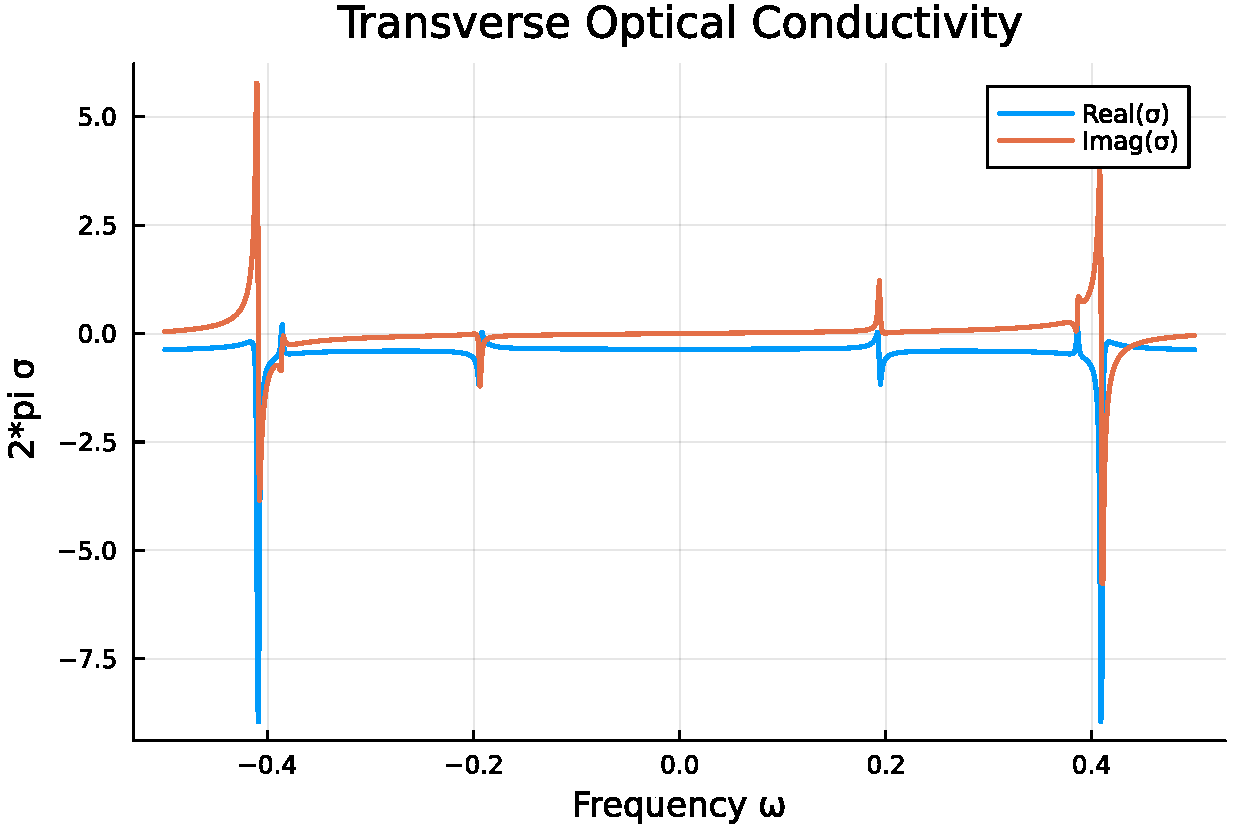
\includegraphics[width=\linewidth]{figures/optical_response/legacy_optical_conductivity_eta_0p001_tag_m0p359.pdf}
  \caption{历史横向响应图；原文件记录了 \(\eta=0.001\) 和尚未解析的标签
  \(-0.359\)。}
\end{subfigure}
\begin{subfigure}{0.48\linewidth}
  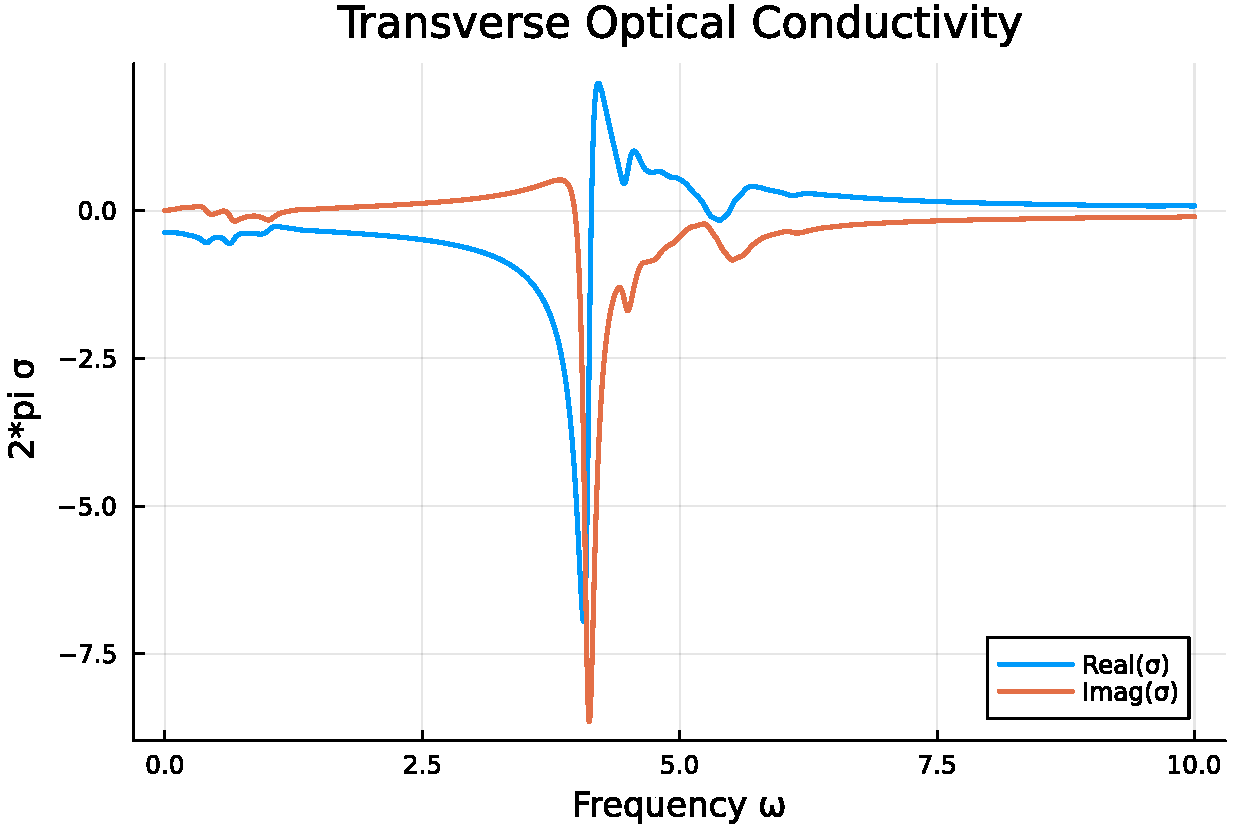
\includegraphics[width=\linewidth]{figures/optical_response/legacy_optical_conductivity_eta_0p065.pdf}
  \caption{记录了 \(\eta=0.065\) 的历史横向响应图。}
\end{subfigure}\hfill
\begin{subfigure}{0.48\linewidth}
  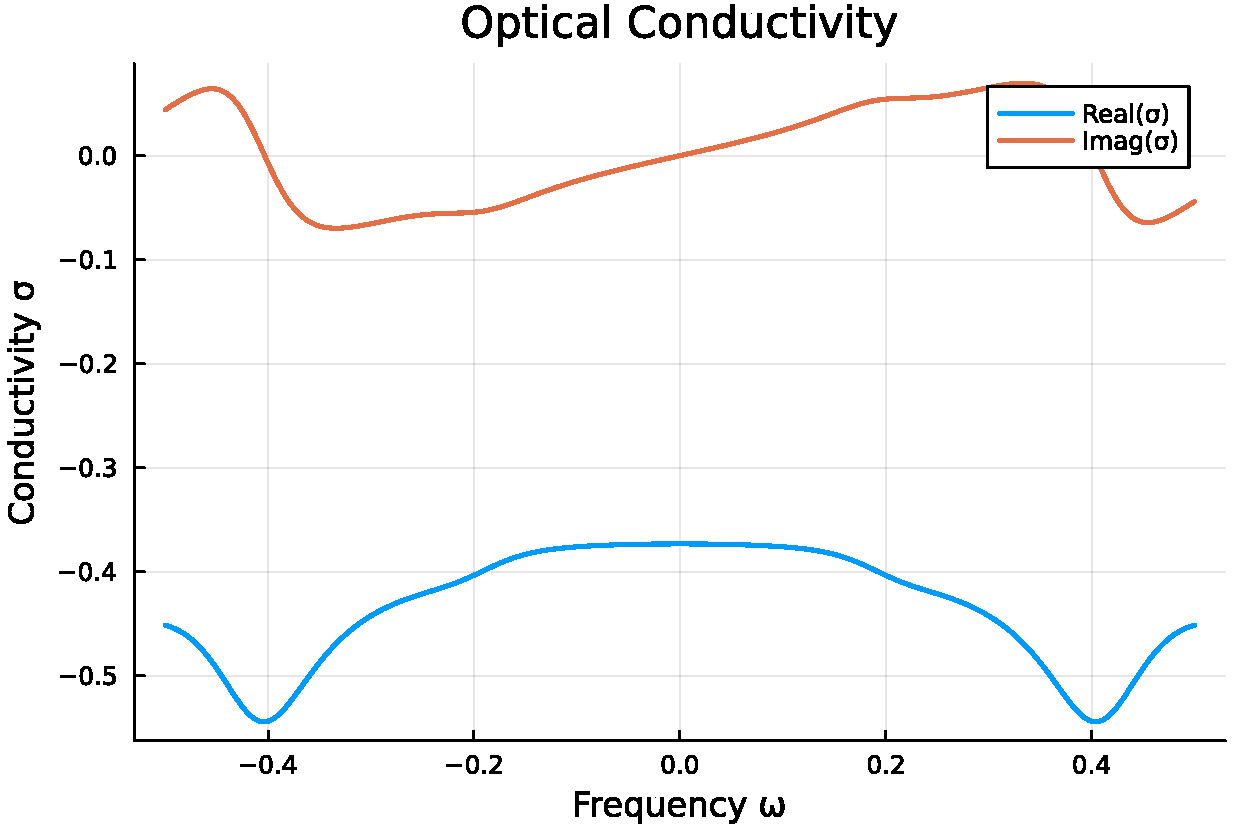
\includegraphics[width=\linewidth]{figures/optical_response/legacy_optical_conductivity_eta_0p065_tag_m0p373.pdf}
  \caption{历史一般响应图；原文件记录了 \(\eta=0.065\) 和尚未解析的标签
  \(-0.373\)。}
\end{subfigure}
\caption{早期线性光电导输出。标签和展宽值直接抄录自图片及文件名；
对于尚未解析的数字标签，这里有意不赋予物理解释。}
\label{fig:legacy-optical-general}
\end{figure}

\begin{figure}[p]
\centering
\begin{subfigure}{0.48\linewidth}
  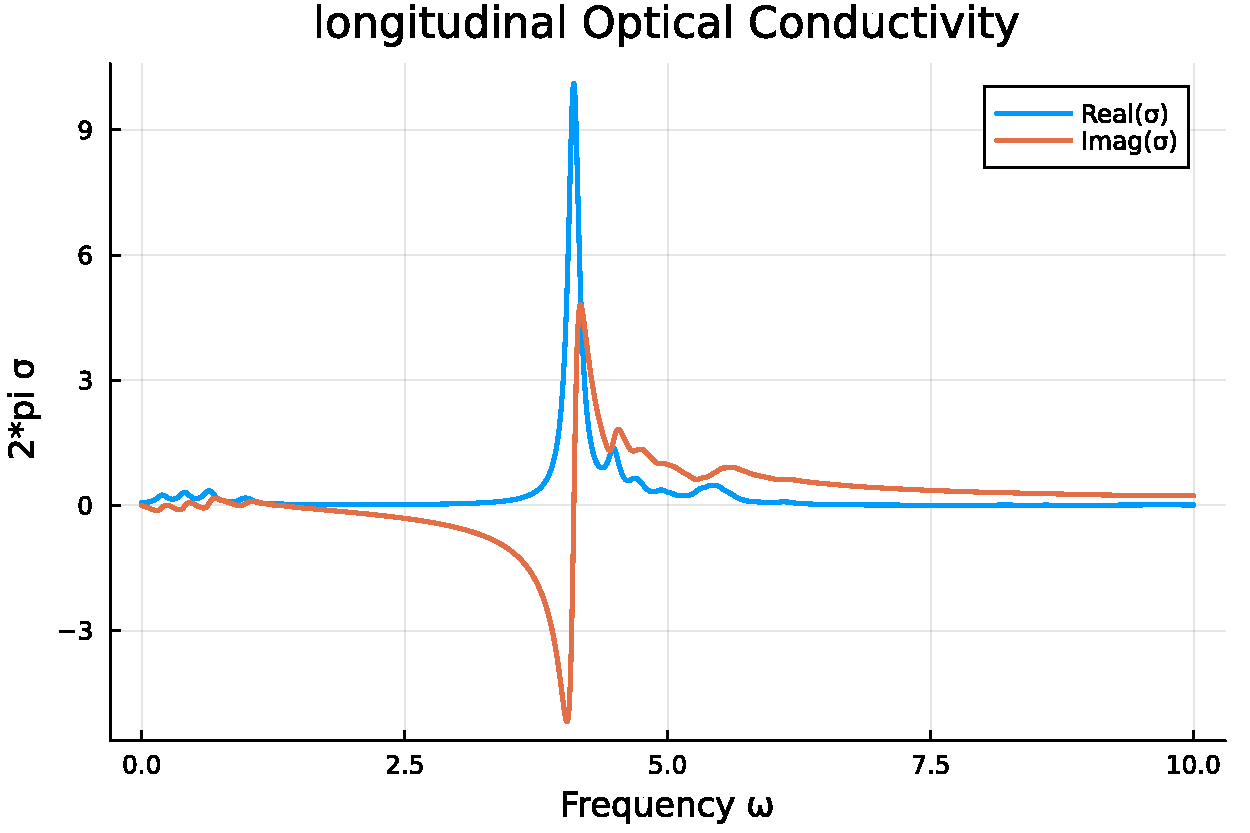
\includegraphics[width=\linewidth]{figures/optical_response/legacy_longitudinal_x.pdf}
  \caption{历史纵向 \(x\) 方向结果。}
\end{subfigure}\hfill
\begin{subfigure}{0.48\linewidth}
  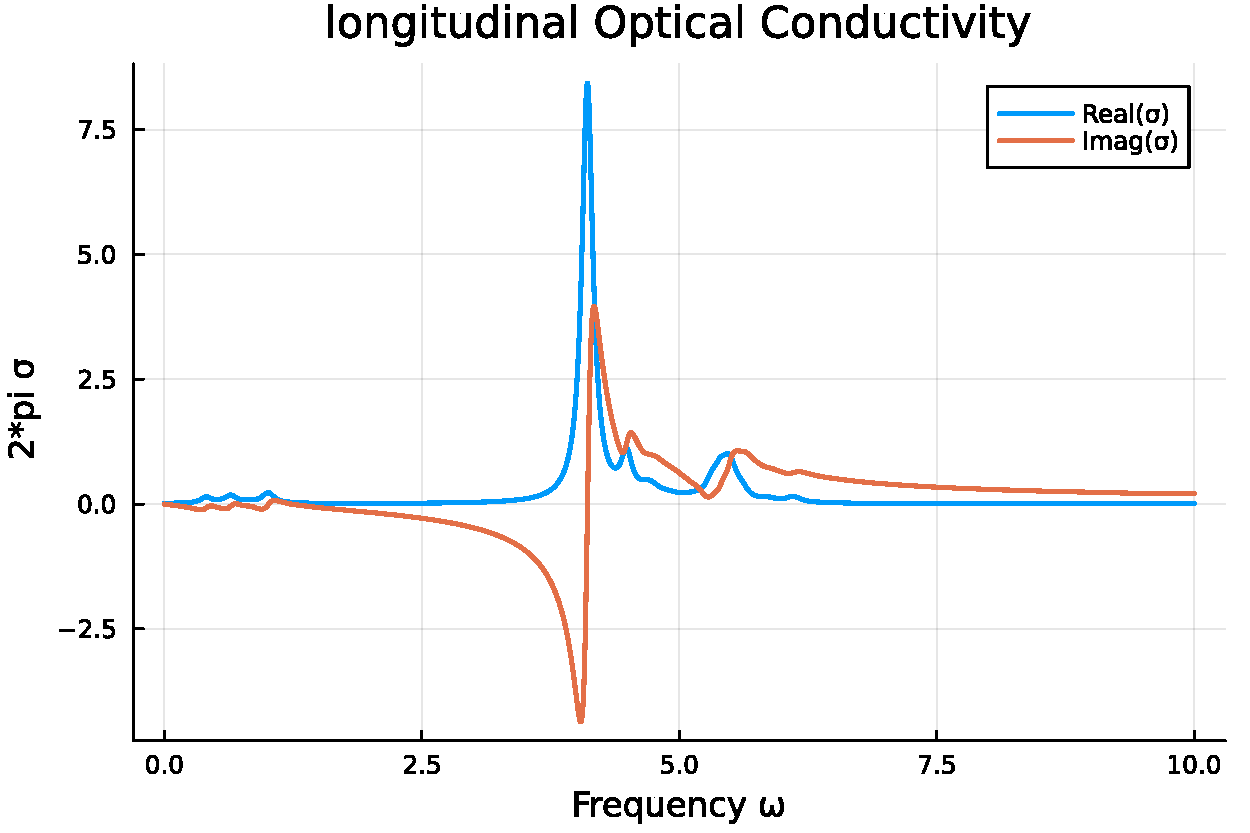
\includegraphics[width=\linewidth]{figures/optical_response/legacy_longitudinal_y.pdf}
  \caption{历史纵向 \(y\) 方向结果。}
\end{subfigure}
\caption{早期纵向 Kubo 响应图。其中实部与虚部是在旧算符和旧面积约定下，
旧 regular 响应表达式 Eq.~\eqref{eq:old-kubo} 的两个分量。}
\label{fig:legacy-optical-longitudinal}
\end{figure}

\clearpage
\subsection{修正后的 \texorpdfstring{\(4\times6\)}{4x6} FCI 基准}

修正后的基准使用 \(4\times6\) torus，取 \(N_p=4\)、动量 sector \(m=2\)、
\(t_1=1\)、\(t_3=0.2\)、\(V_1=1\)、\(V_2=V_3=0\)。频率网格为
\(0:0.001:10\)，展宽为 \(\eta=0.065\)。

\begin{table}[h]
\centering
\caption{修正后的有限 torus 光学响应基准。}
\begin{tabular}{lr}
\toprule
物理量 & 数值 \\
\midrule
\(E_g\) & \(-9.313575887962\) \\
\(\langle K_{xx}\rangle\) & \(4.47923524291\) \\
\(\lVert QJ_x\lvert g\rangle\rVert^2\) & \(10.8443081433\) \\
\(D_{xx}\) & \(-0.885036768331\) \\
Regular 主峰 \((\omega,\operatorname{Re}\sigma_{xx}^{\mathrm{reg}})\) &
\((4.107,9.34982602717)\) \\
最终 response 维数 & \(892\) \\
Exact--Lanczos 缩放最大误差 & \(5.5927404437300286\times10^{-14}\) \\
\bottomrule
\end{tabular}
\end{table}

下图蓝色 exact 曲线由有限动量 sector 的完整 ED 本征态求和
Eq.~\eqref{eq:exact-resolvent} 得到，并不是换了标签的 Lanczos 数据。
最终 response-Lanczos 结果画为较细的红色虚线，因此即使两者在绘图精度内一致，
也可以从虚线间隙中看到蓝色 exact 曲线。每个 inset 用对数坐标显示逐点的
exact--Lanczos 绝对差值。两者缩放最大误差只有
\(5.59\times10^{-14}\)，所以主图中蓝线若不明显，是因为两条曲线重合并相互遮盖，
而不是因为没有计算或绘制 exact 结果。regular 实部的主吸收峰位于
\(\omega=4.107\)，峰高为 \(9.349826\)。

这个 FCI 数据的基态位于 \(m=2\)；另两个近简并低能态位于 \(m=6,10\)，
三态能量散布约为 \(0.00555\)，三态流形到第四个低能态的有限尺寸间隔约为
\(0.09424\)。实空间密度在每个 site 上均为 \(1/6\)。均匀电流算符 \(J_x\)
不改变晶格总动量，因此从 \(m=2\) 基态计算的 \(\sigma_{xx}\) 只看到同一 sector
中具有非零电流矩阵元的 bright 中性激发。\(\omega=4.107\) 是这里最强的
current-active 激发，而不是三态流形的劈裂或完整 many-body gap；光电导本身也不直接
显示三重拓扑基态流形、many-body Chern number 或分数量子化 Hall 响应。

\begin{figure}[p]
\centering
\begin{subfigure}{0.48\linewidth}
  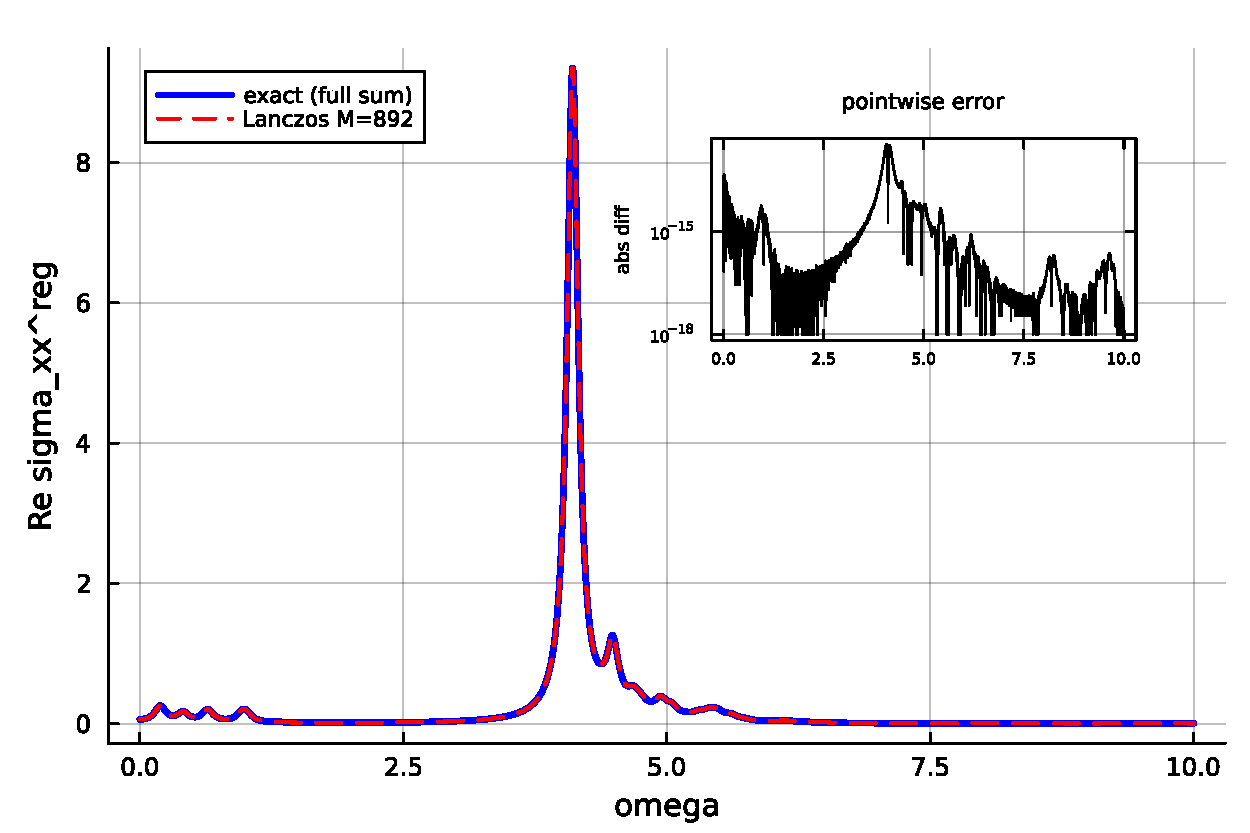
\includegraphics[width=\linewidth]{figures/optical_response/corrected_sigma_xx_regular_real.pdf}
  \caption{\(\operatorname{Re}\sigma_{xx}^{\mathrm{reg}}\).}
\end{subfigure}\hfill
\begin{subfigure}{0.48\linewidth}
  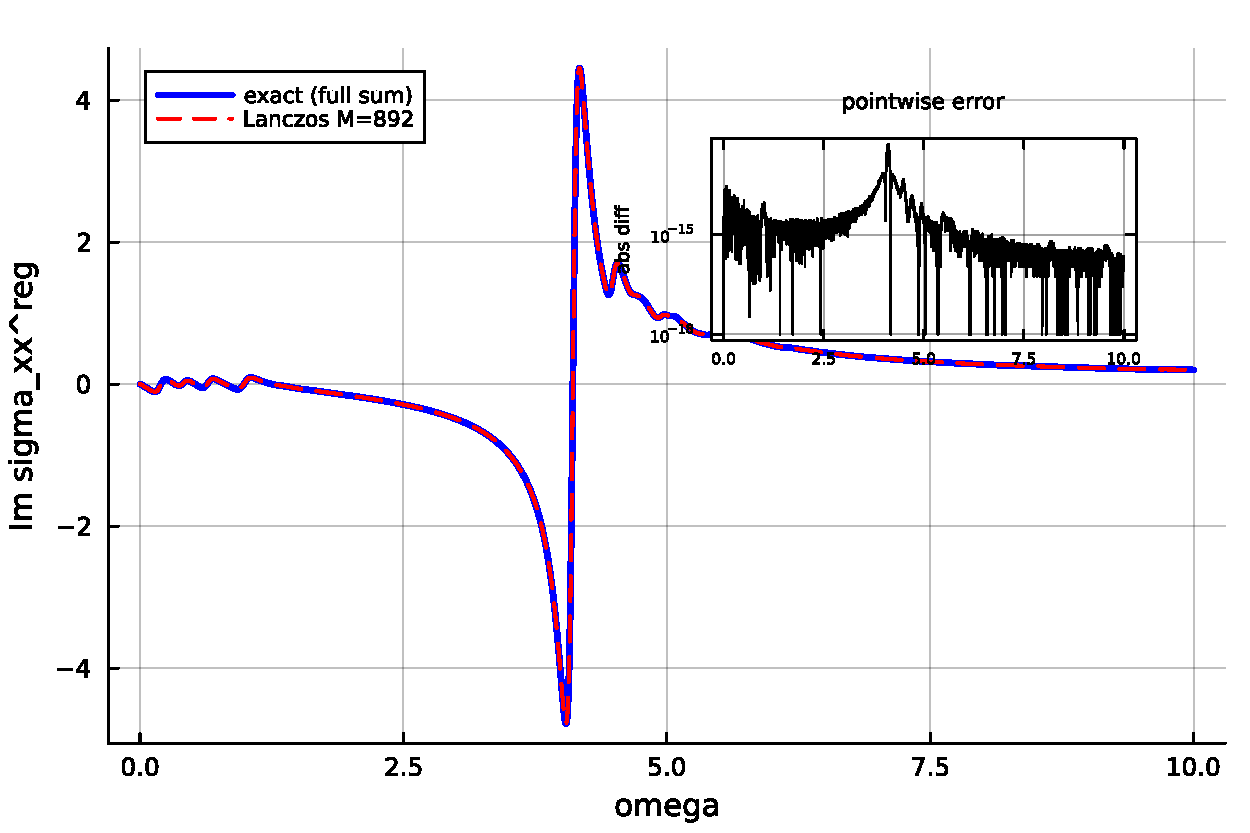
\includegraphics[width=\linewidth]{figures/optical_response/corrected_sigma_xx_regular_imag.pdf}
  \caption{\(\operatorname{Im}\sigma_{xx}^{\mathrm{reg}}\).}
\end{subfigure}
\par\medskip
\begin{subfigure}{0.48\linewidth}
  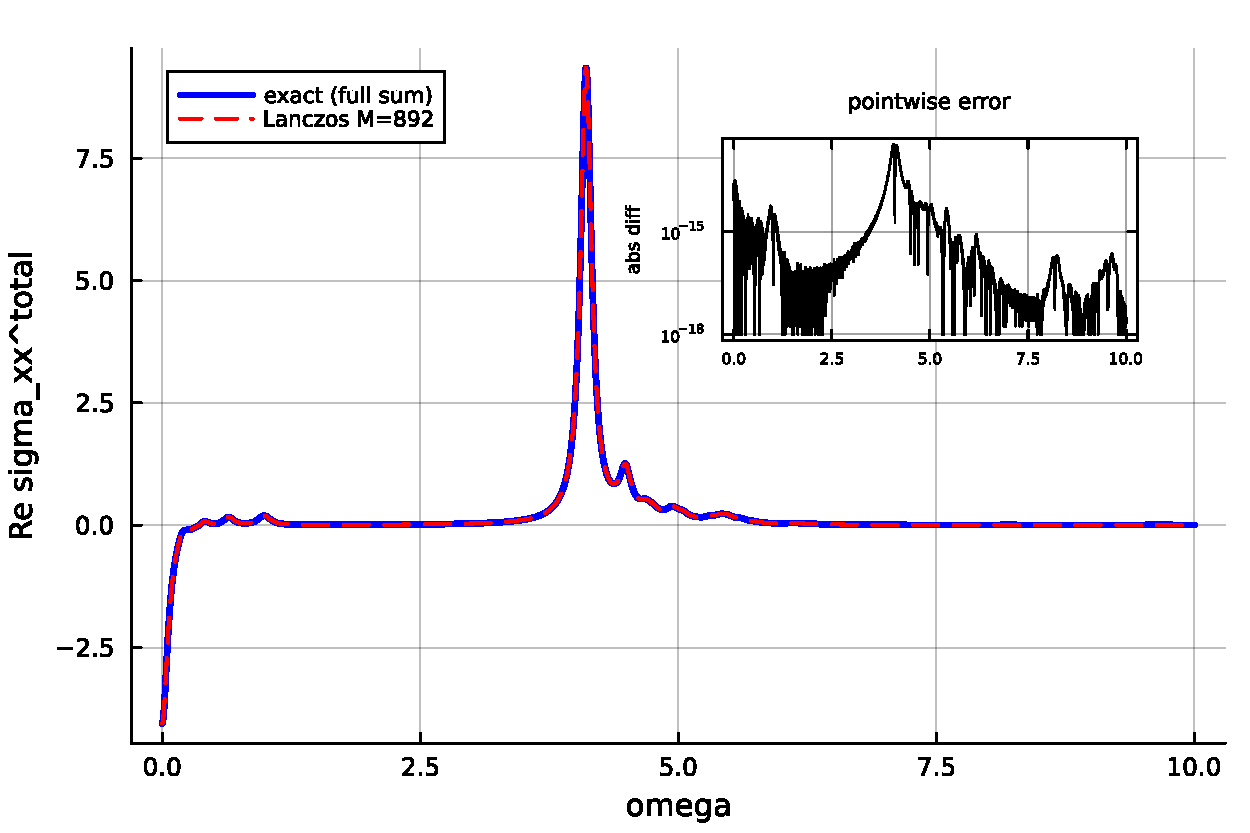
\includegraphics[width=\linewidth]{figures/optical_response/corrected_sigma_xx_total_real.pdf}
  \caption{\(\operatorname{Re}\sigma_{xx}^{\mathrm{total}}\).}
\end{subfigure}\hfill
\begin{subfigure}{0.48\linewidth}
  
\includegraphics[width=\linewidth]{figures/optical_response/corrected_sigma_xx_total_imag.pdf}
  \caption{\(\operatorname{Im}\sigma_{xx}^{\mathrm{total}}\).}
\end{subfigure}
\caption{修正后的四个纵向光电导分量。每幅图中，粗蓝色实线是完整 exact
本征态求和，细红色虚线是 \(M=892\) 的 response-Lanczos；inset 表示二者逐点
绝对差值。两种方法都是 ED，并计算相同的 Kubo resolvent。}
\label{fig:corrected-optical-benchmark}
\end{figure}

\begin{figure}[p]
\centering
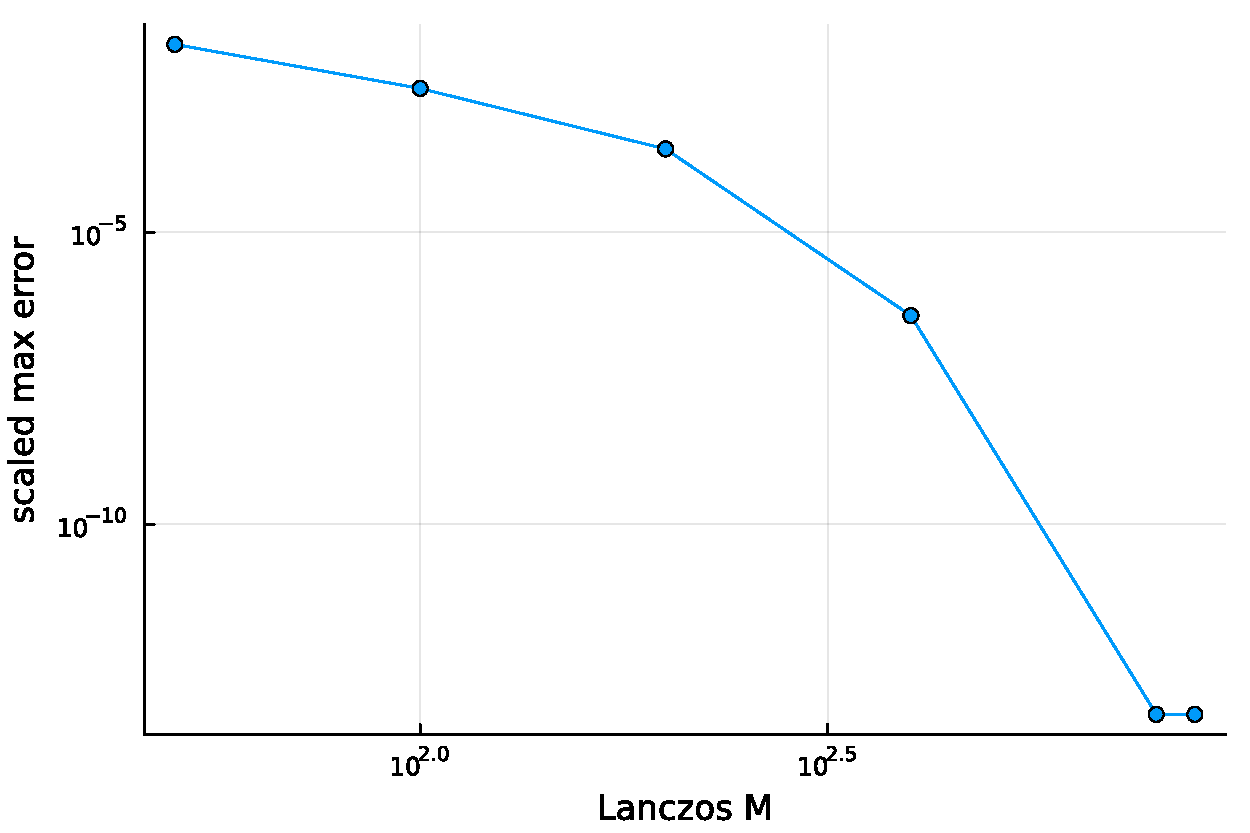
\includegraphics[width=0.62\linewidth]{figures/optical_response/corrected_lanczos_convergence.pdf}
\caption{regular 电导的缩放最大误差随 response 维数的收敛。}
\label{fig:corrected-optical-convergence}
\end{figure}

\clearpage
\subsection{强耦合三周期 CDW 的 30-site ED 能谱}

当前光学响应使用倾斜 30-site torus 上的强耦合三周期 CDW 参数点。完整模型与
粒子数参数为
\[
  N_s=30,\qquad N_{\mathrm{uc}}=15,\qquad N_p=12,
\]
\[
  t_1=1,\qquad t_3=0.2,\qquad V_1=100,\qquad V_2=V_3=0.
\]
这里 \(N_p/N_s=2/5\)，若以两 site unit cell 的数目计，则
\(N_p/N_{\mathrm{uc}}=4/5\)。多节点 ED 将 Hilbert 空间分解为
\(k=0,\ldots,14\) 共 15 个动量 sector，并在每个 sector 中使用 Lanczos
保存最低 8 个本征值。因此图~\ref{fig:phc30-manybody-spectrum} 共包含
\(15\times8=120\) 个能级，纵轴均为相对全局基态的 \(E-E_0\)。全局基态能量为
\[
  E_0=594.8436843931768,
\]
最低的两个 sector 为 \(k=5\) 和 \(k=10\)，在保存精度内具有相同能量；
\(k=0\) 的最低态位于 \(E-E_0=0.0001245629\)。因此基态流形是
\(k=0,5,10\) 的三重 CDW 基态，其有限尺寸内部劈裂为
\[
  E_3-E_1=0.0001245629.
\]
第 4 个能级位于 \(k=2\)（并与 \(k=13\) 对称），其能量为
\[
  E_4-E_1=0.0213937117,
\]
所以三重基态到第 4 态的有限尺寸间隔为
\[
  E_4-E_3=0.0212691488.
\]
从第 4 态到第 15 态的其余 12 个态分布在
\(E-E_0=0.0213937117\)--\(0.0287121891\)，它们是低能激发，不能作为
15 重基态简并来解释。

\begin{figure}[H]
\centering
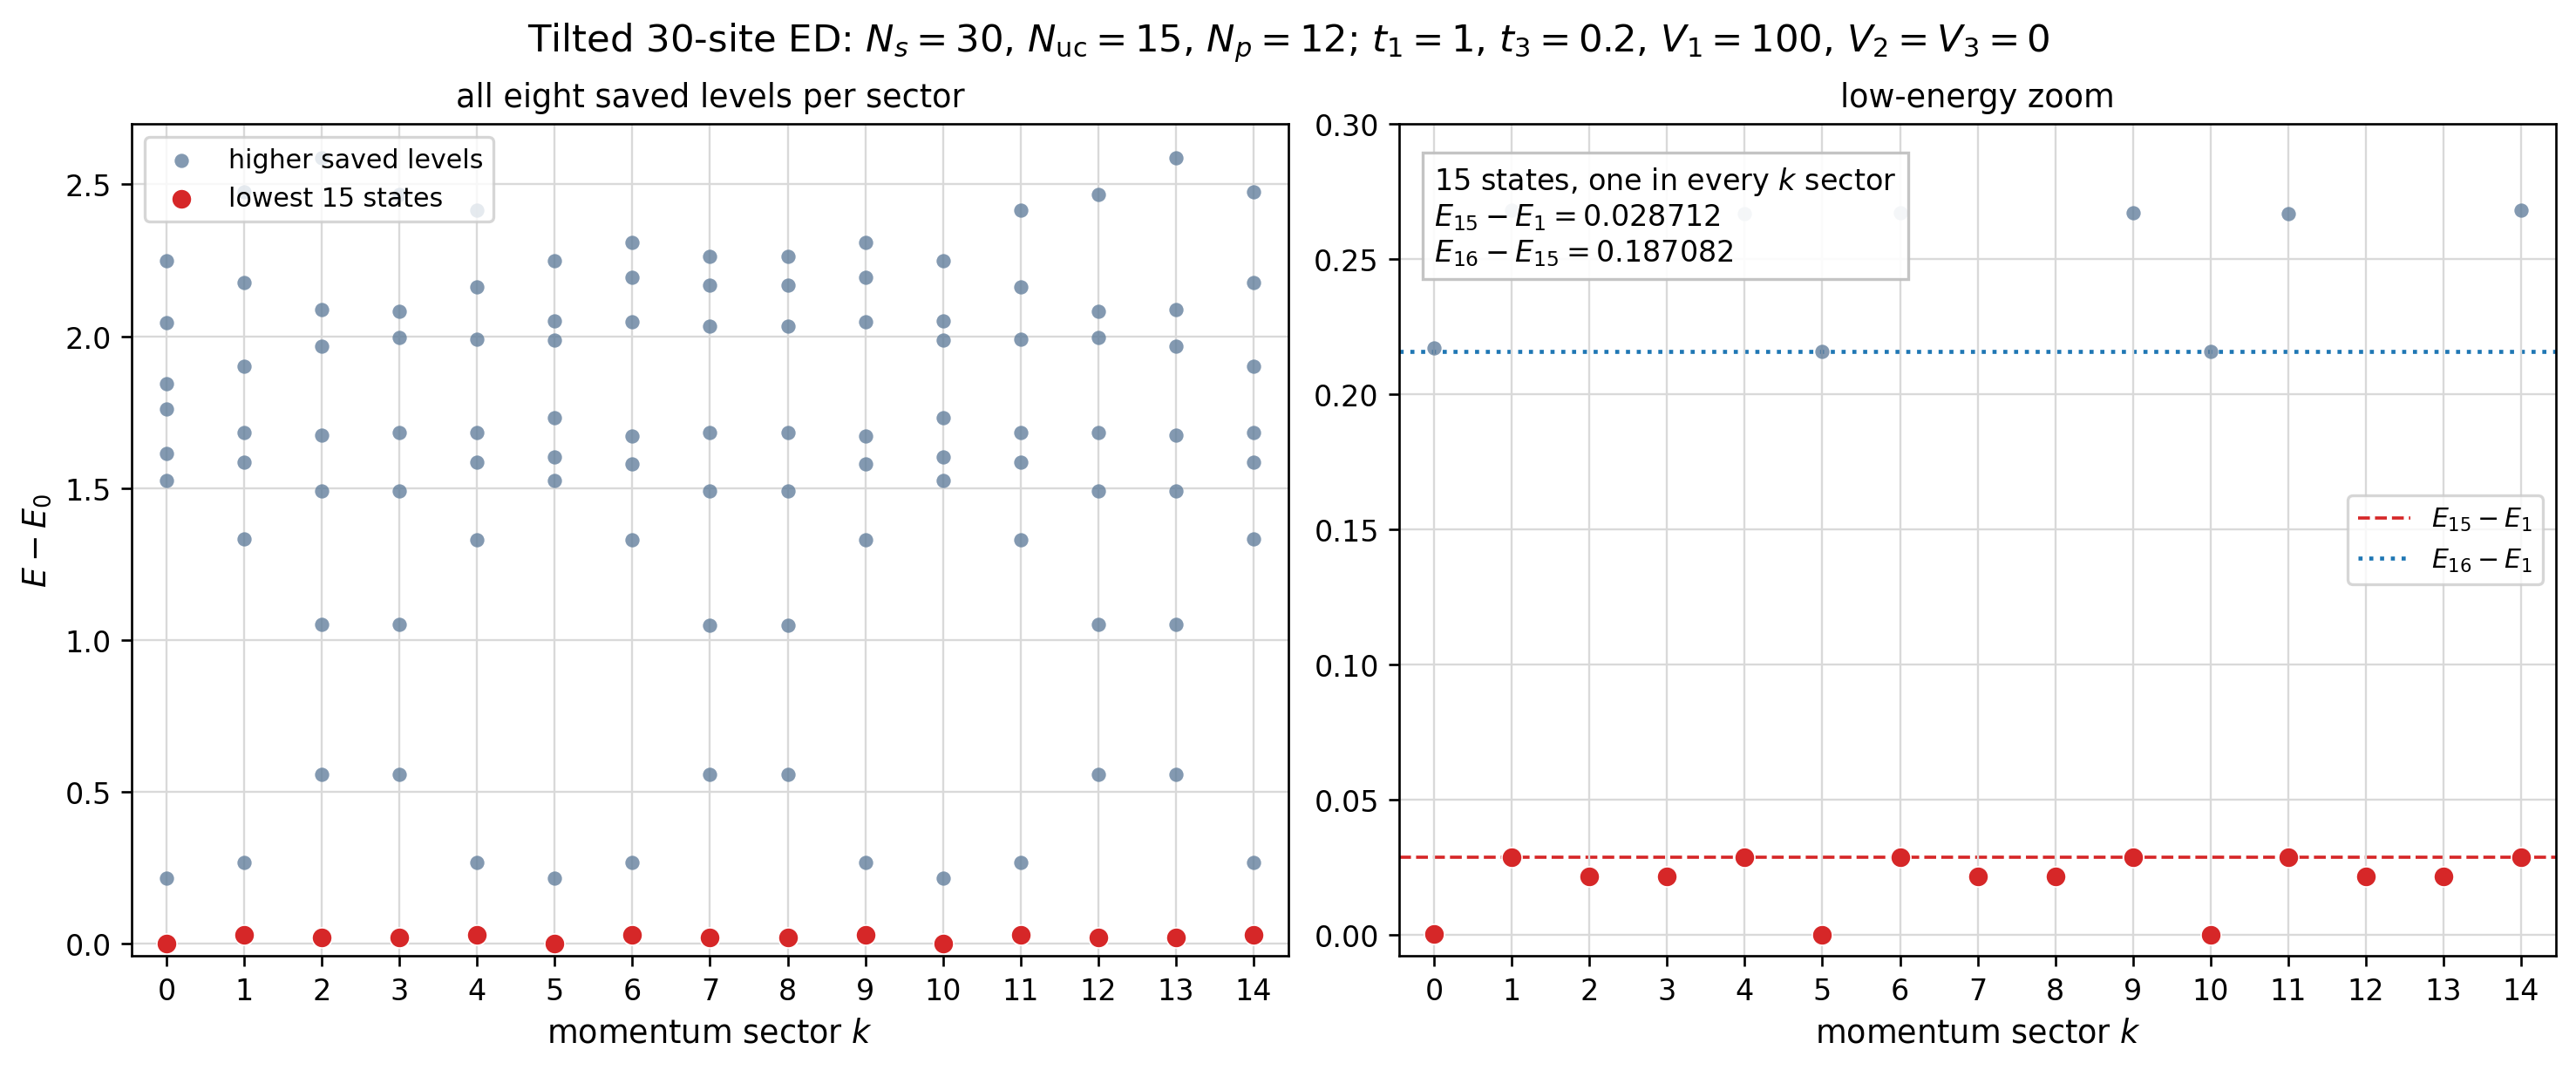
\includegraphics[width=0.96\linewidth]{figures/optical_response/phc30_manybody_spectrum.png}
\caption{强耦合三周期 CDW 参数点的 30-site 多体 ED 能谱。左图画出每个
动量 sector 保存的最低 8 个能级；右图放大低能区。红色点是 \(k=0,5,10\)
三重基态，蓝灰色点是保存的激发态。红色虚线标记三态宽度 \(E_3-E_1\)，
蓝色点线标记第 4 态能量 \(E_4-E_1\)。数据来自多节点 ED，而不是
response-Lanczos 光学迭代。}
\label{fig:phc30-manybody-spectrum}
\end{figure}

三重基态的静态结构因子由同一组多节点 ED 保存波函数直接计算。定义为
\[
  N(\mathbf q)=\frac{1}{N_{\mathrm{uc}}}
  \left\langle
  \left|\sum_j e^{i\mathbf q\cdot\mathbf R_j}
  (n_j-\bar n)\right|^2
  \right\rangle ,
\]
这里采用原胞归一化 \(N_{\mathrm{uc}}=15\)，并使用生成
\(\texttt{partial\_*.jld2}\) 时与 unit-cell 平移字符一致的 TiltedLat30 Fourier 网格；
程序中的 legacy 标签只用于兼容旧分组文件布局。计算仍是
ED：程序从 \(k=0,5,10\) 三个保存的基态向量重建相应动量基，并利用
平移轨道代表元求和；这一步不使用 DMRG。

三态都在 \(q=5,10\) 出现两个等高主峰。具体数值为
\[
\begin{array}{c|cc}
\text{基态 sector} & N(q=5) & N(q=10)\\
\hline
0  & 1.441939701645 & 1.441939701645\\
5  & 1.441747323260 & 1.441747323260\\
10 & 1.441752041980 & 1.441752041980
\end{array}
\]
三态平均峰高为 \(1.441813022295\)。每个向量的范数为 1，粒子数检验为 12。
三态曲线几乎完全重合，\(q=5,10\) 双峰直接确认该参数点的三周期 CDW，
并与能谱中的 \(k=0,5,10\) 三重基态相互对应。

\begin{figure}[H]
\centering
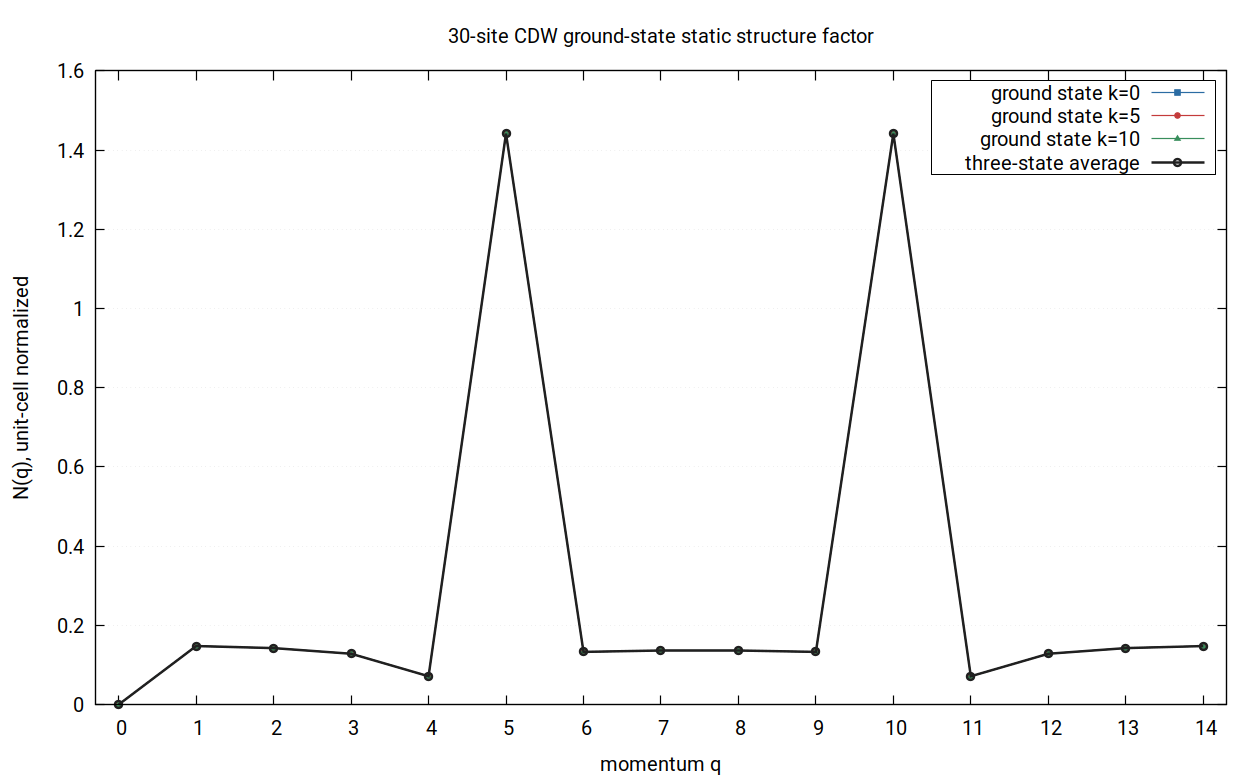
\includegraphics[width=0.82\linewidth]{figures/optical_response/phc30_cdw_structure_factor.png}
\caption{\(V_1=100,V_2=V_3=0\) 强耦合 CDW 三重基态的静态结构因子。
蓝、红、绿细线分别来自 \(k=0,5,10\) 基态，黑色粗线是三态平均。纵轴采用
原胞归一化 \(1/N_{\mathrm{uc}}\)；\(q=5,10\) 的 Bragg 双峰表明周期三密度序。}
\label{fig:phc30-cdw-structure-factor}
\end{figure}

这张能谱也说明后面的光电导不能被理解为完整低能谱。均匀电流算符 \(J_x\)
保持晶格总动量，因此从 \(m=5\) 或 \(m=10\) 基态出发时，只会直接耦合到同一
sector 中电流矩阵元非零的激发。两个 sector 的第一个同 sector 激发位于
\(\Delta E=0.2157939408\)，但它在 \(\sigma_{xx}\) 中没有形成可见强峰；
后文的主要光学峰则对应 \(\Delta E=1.5245875\) 和 \(2.2476085\) 的
current-active 激发。

\clearpage
\subsection{30-site 强耦合 CDW 正式响应计算}

大系统响应使用旧有的倾斜 30-site torus，保存的基态由多节点 ED 程序得到。
计算保持该数据原有且与平移字符一致的 Fourier 网格和 hopping 约定不变。三重基态中，
现有光学数据只计算了严格简并的 \(m=5\) 与 \(m=10\) 两个 sector；尚未计算
\(m=0\) 的响应。模型和响应参数为
\[
  N_s=30,\quad N_p=12,\quad t_1=1,\quad t_3=0.2,\quad
  V_1=100,\quad V_2=V_3=0,
\]
\[
  \eta=0.065,\qquad \omega=0:0.002:10,\qquad M=600.
\]
每个动量 sector 的维数为 \(5{,}766{,}201\)，稀疏 Hamiltonian 含有
\(435{,}245{,}593\) 个非零矩阵元。程序只构造一次稀疏 Hamiltonian，随后使用
多线程 response-Lanczos 迭代；不求出也不保存全部激发态向量。因此，本节结果是
多节点/多线程 ED 加 response-Lanczos 所得的光电导，不是 DMRG 动力学响应。

\begin{table}[H]
\centering
\small
\caption{30-site 强耦合 CDW response-Lanczos 计算的诊断量。}
\begin{tabular}{lrr}
\toprule
物理量 & \(m=5\) & \(m=10\) \\
\midrule
\(E_g\) & \(594.8436843931768\) & \(594.8436843931768\) \\
\(\lVert H|g\rangle-E_g|g\rangle\rVert\) &
\(2.96845\times10^{-12}\) & \(2.41234\times10^{-12}\) \\
\(\lVert QJ_x|g\rangle\rVert^2\) &
\(31.2733061902965\) & \(31.2733061902929\) \\
\(\langle K_{xx}\rangle\) & \(3.32417392623293\) & \(3.32417392623468\) \\
\(D_{xx}\) & \(-0.481293569882233\) & \(-0.481293569881193\) \\
Lanczos 步数 & 600 & 600 \\
\bottomrule
\end{tabular}
\end{table}

两个 sector 的曲线在绘图精度内一致。在全部 5001 个频率点上，regular/total
实部与虚部中的最大逐点差值为 \(3.22\times10^{-7}\)，Drude 分量的最大差值为
\(3.87\times10^{-12}\)。因此图中的两条线表示对称相关的 \(m=5\) 与 \(m=10\)
sector 给出的同一物理响应，而不是 exact 与 Lanczos 的算法对照。作为内部收敛检验，
将保存的 \(m=10\) continued fraction 从 \(M=600\) 截断至 \(M=500\) 后，
regular 电导的最大绝对变化为 \(1.6620\times10^{-4}\)，RMS 差值为
\(1.5587\times10^{-5}\)；在信号大于 \(10^{-6}\) 的区域，最大相对差值为
\(8.03\times10^{-4}\)。

在 \(\operatorname{Re}\sigma_{xx}^{\mathrm{reg}}\) 中，两个最主要的吸收峰为
\[
  (\omega,\operatorname{Re}\sigma_{xx}^{\mathrm{reg}})
  \simeq(1.524,4.55784),\qquad(2.248,1.33201).
\]
较弱结构位于 \(\omega\simeq1.998,2.986,4.770\)，对应峰高约为
\(0.3516,0.1401,0.07835\)。这些峰给出均匀电流算符 \(J_x\) 能够耦合的
current-active 中性激发。由于 \(J_x\) 保持晶格总动量，光电导只探测与基态同一
sector 且电流矩阵元非零的激发：其他 sector 中 \(0.02\) 量级的低能态不会直接出现，
同一 sector 中 \(\Delta E\simeq0.2158\) 的激发也没有形成可见强峰，说明它对
\(J_x\) 是 optical-dark 或仅有很小矩阵元。因此首个强吸收峰给出 optical gap，
不能直接当作完整的 many-body spectral gap。
在同一 \(m=5/10\) sector 的能谱中，\(\Delta E=1.5245875\) 与
\(2.2476085\) 的激发分别对应上面的两个主要光学峰；这项对应关系确认了峰位来自
same-sector 的 current-active 本征激发。

四幅图的含义如下：regular 实部给出经 \(\eta=0.065\) 展宽的有限频率吸收；
regular 虚部是其色散响应；total 实部在 regular 吸收上加入展宽的 Drude 贡献；
total 虚部还包含相应的低频反应性 Drude 极点。

\begin{figure}[p]
\centering
\begin{subfigure}{0.48\linewidth}
  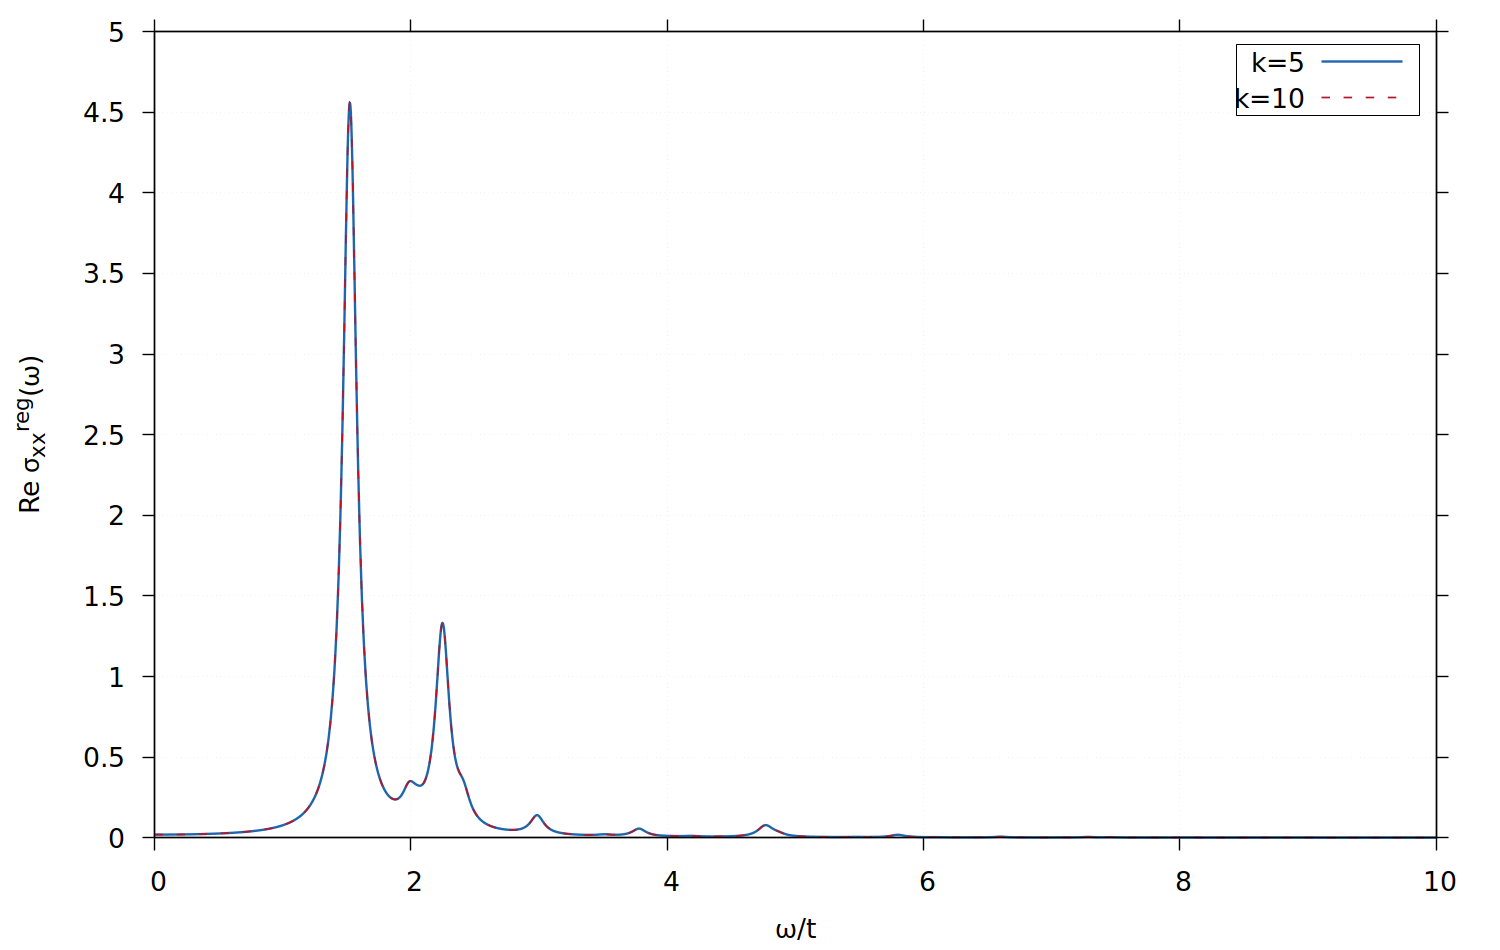
\includegraphics[width=\linewidth]{figures/optical_response/phc30_sigma_xx_regular_real.png}
  \caption{\(\operatorname{Re}\sigma_{xx}^{\mathrm{reg}}\).}
\end{subfigure}\hfill
\begin{subfigure}{0.48\linewidth}
  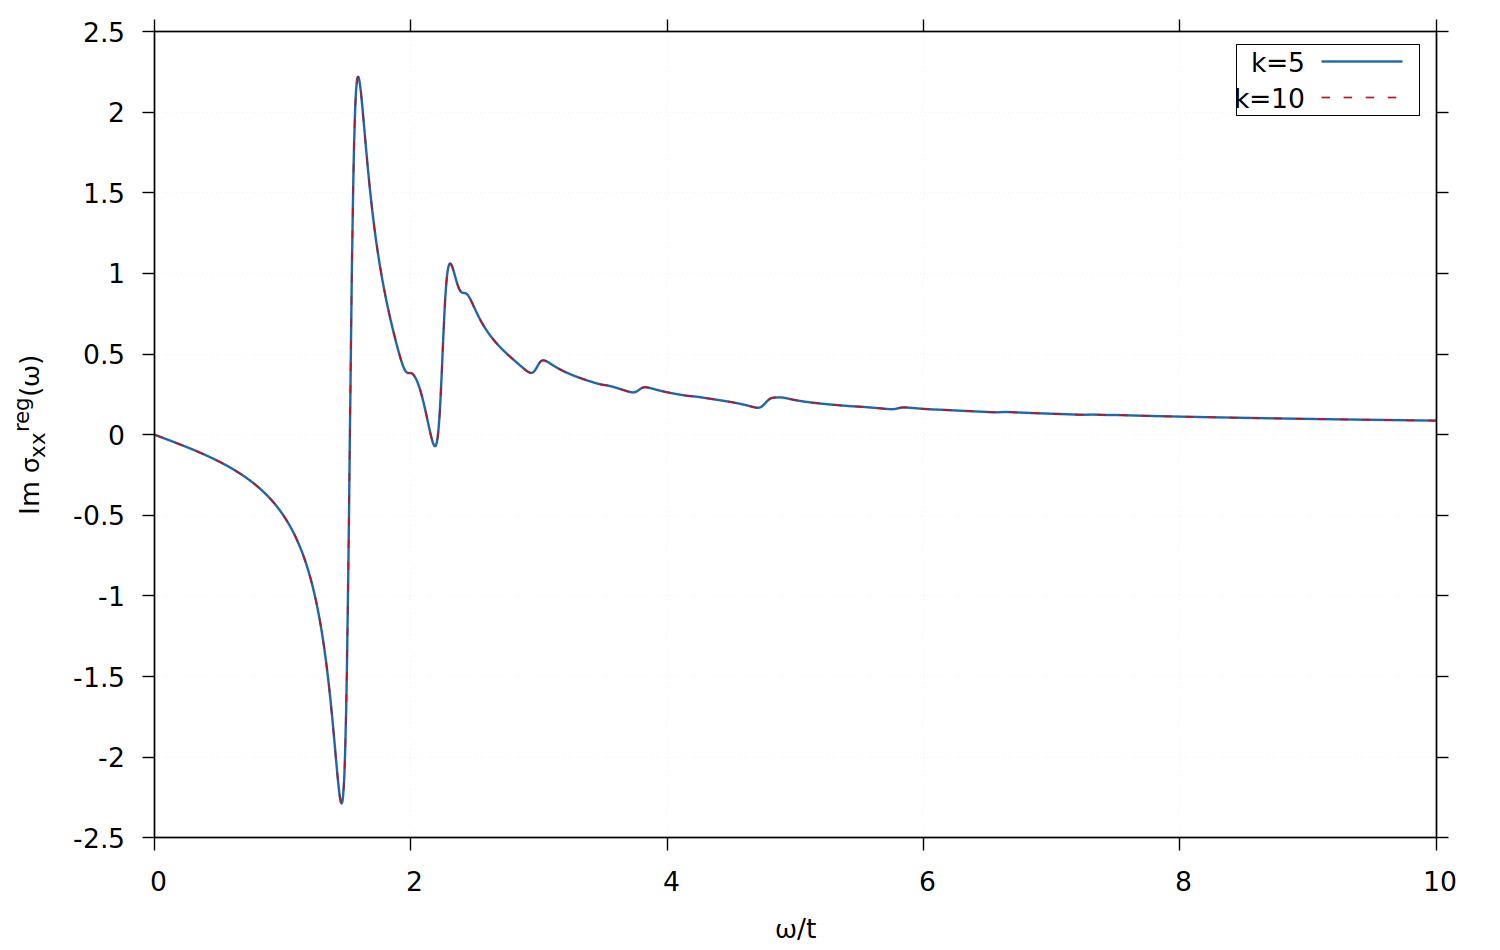
\includegraphics[width=\linewidth]{figures/optical_response/phc30_sigma_xx_regular_imag.png}
  \caption{\(\operatorname{Im}\sigma_{xx}^{\mathrm{reg}}\).}
\end{subfigure}
\par\medskip
\begin{subfigure}{0.48\linewidth}
  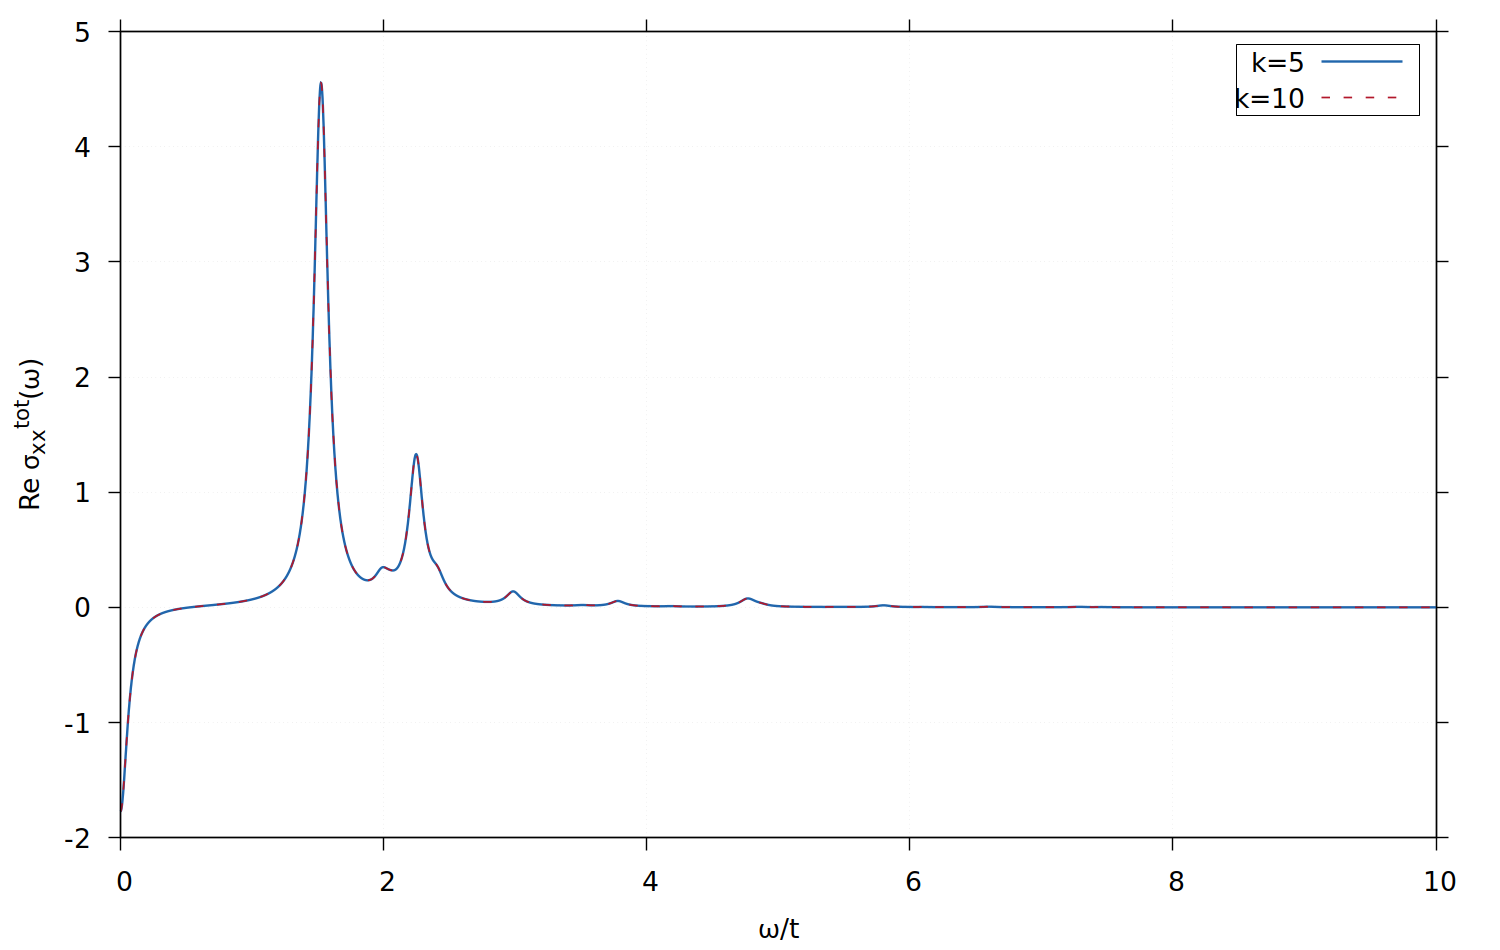
\includegraphics[width=\linewidth]{figures/optical_response/phc30_sigma_xx_total_real.png}
  \caption{\(\operatorname{Re}\sigma_{xx}^{\mathrm{total}}\).}
\end{subfigure}\hfill
\begin{subfigure}{0.48\linewidth}
  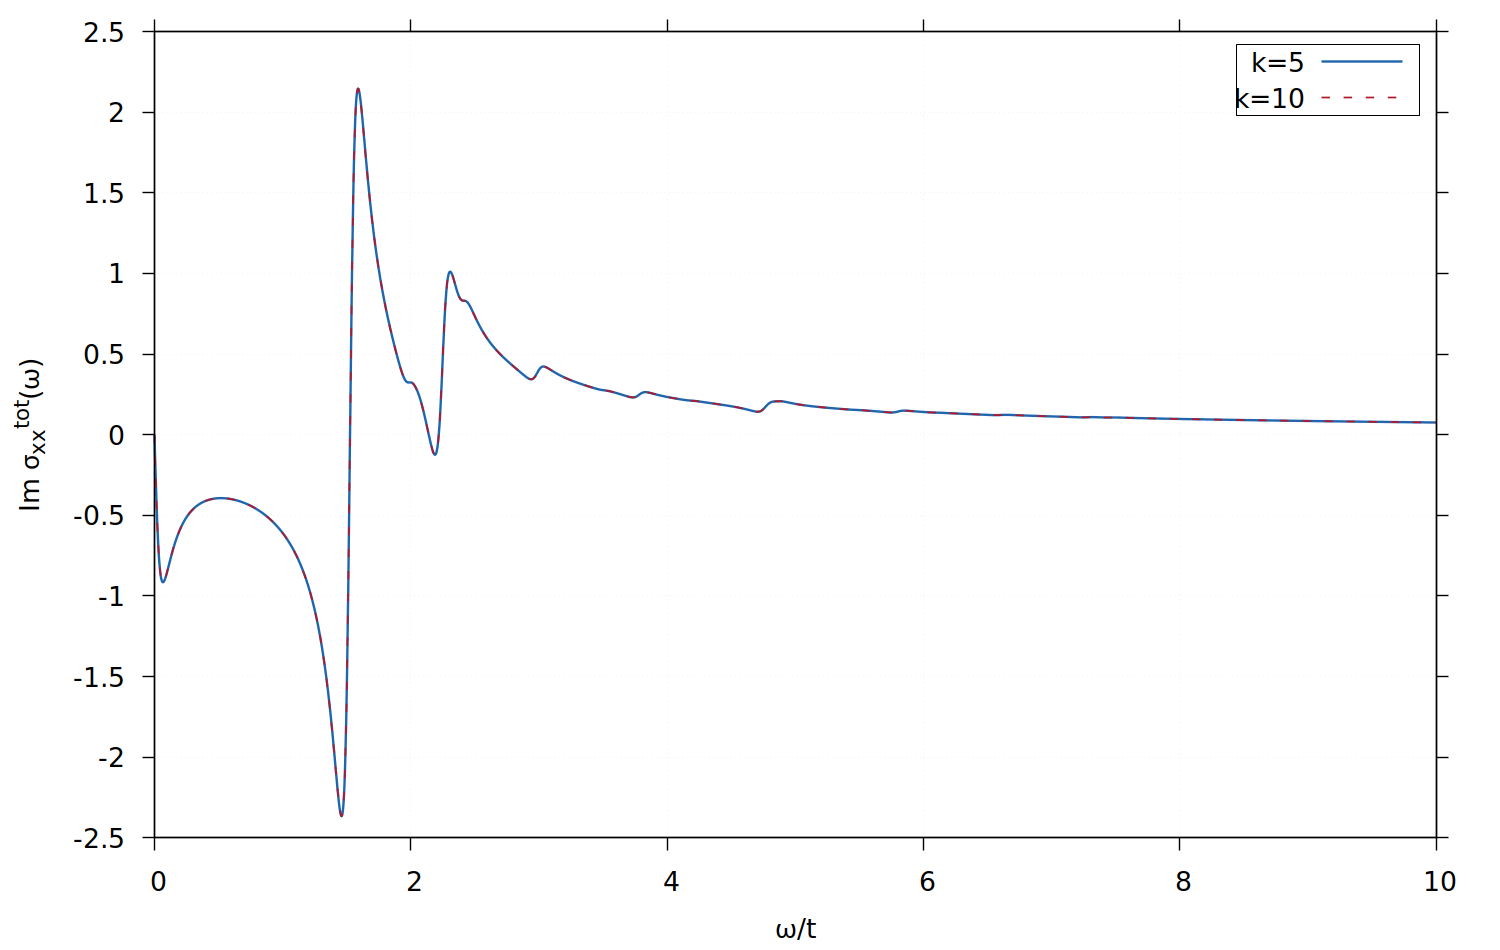
\includegraphics[width=\linewidth]{figures/optical_response/phc30_sigma_xx_total_imag.png}
  \caption{\(\operatorname{Im}\sigma_{xx}^{\mathrm{total}}\).}
\end{subfigure}
\caption{30-site 强耦合 CDW 的纵向光电导。蓝色实线和红色虚线分别是独立计算的
\(m=5\) 与 \(m=10\) 简并 sector；两者近乎完全重合是数值一致性检验，并不是
exact-spectrum 对照。低频处展宽后 total 贡献为负，来自表中有限 twist 下的
\(D_{xx}\)，应结合前述有限尺寸曲率限制解释。}
\label{fig:phc30-optical-response}
\end{figure}

\clearpage
\subsection{温和参数的 30-site CDW 态}

回到较温和的相互作用参数，计算采用与强耦合结果相同的倾斜 30-site torus：
\[
  N_s=30,\qquad N_{\mathrm{uc}}=15,\qquad N_p=12,
\]
\[
  t_1=1,\qquad t_3=0.2,\qquad V_1=10,\qquad V_2=V_3=2.
\]
多节点 ED 在 \(k=0,\ldots,14\) 的每个动量 sector 中保存最低 8 个能级和最低态
波函数，所以完整能谱仍包含 \(15\times8=120\) 个能级。全局基态能量为
\[
  E_0=121.990425977706.
\]
最低 15 态恰好在每个 sector 中各有一态，其流形宽度以及流形上方的间隔为
\[
  E_{15}-E_1=0.034430068375,\qquad
  E_{16}-E_1=0.594687763692,
\]
\[
  E_{16}-E_{15}=0.560257695317.
\]
因此第 15 至 16 态的间隔约为流形内部宽度的 16.3 倍；在这个有限系统上，
最低 15 态构成清楚隔离的低能流形。最低的 \(k=10\) 与 \(k=5\) 两态在保存精度内
简并；下一对 \(k=12,3\) 位于 \(E-E_0=0.009268092715\)，其余低能态一直分布到
\(E-E_0=0.034430068375\)。因此这 15 态不能解释为 15 重简并基态，更不能仅由
态数推出分数拓扑简并。结合下述 \(q=5,10\) Bragg 峰，本参数点归类为 CDW；
这 15 态应称为隔离的 CDW 低能流形。

\begin{figure}[H]
\centering
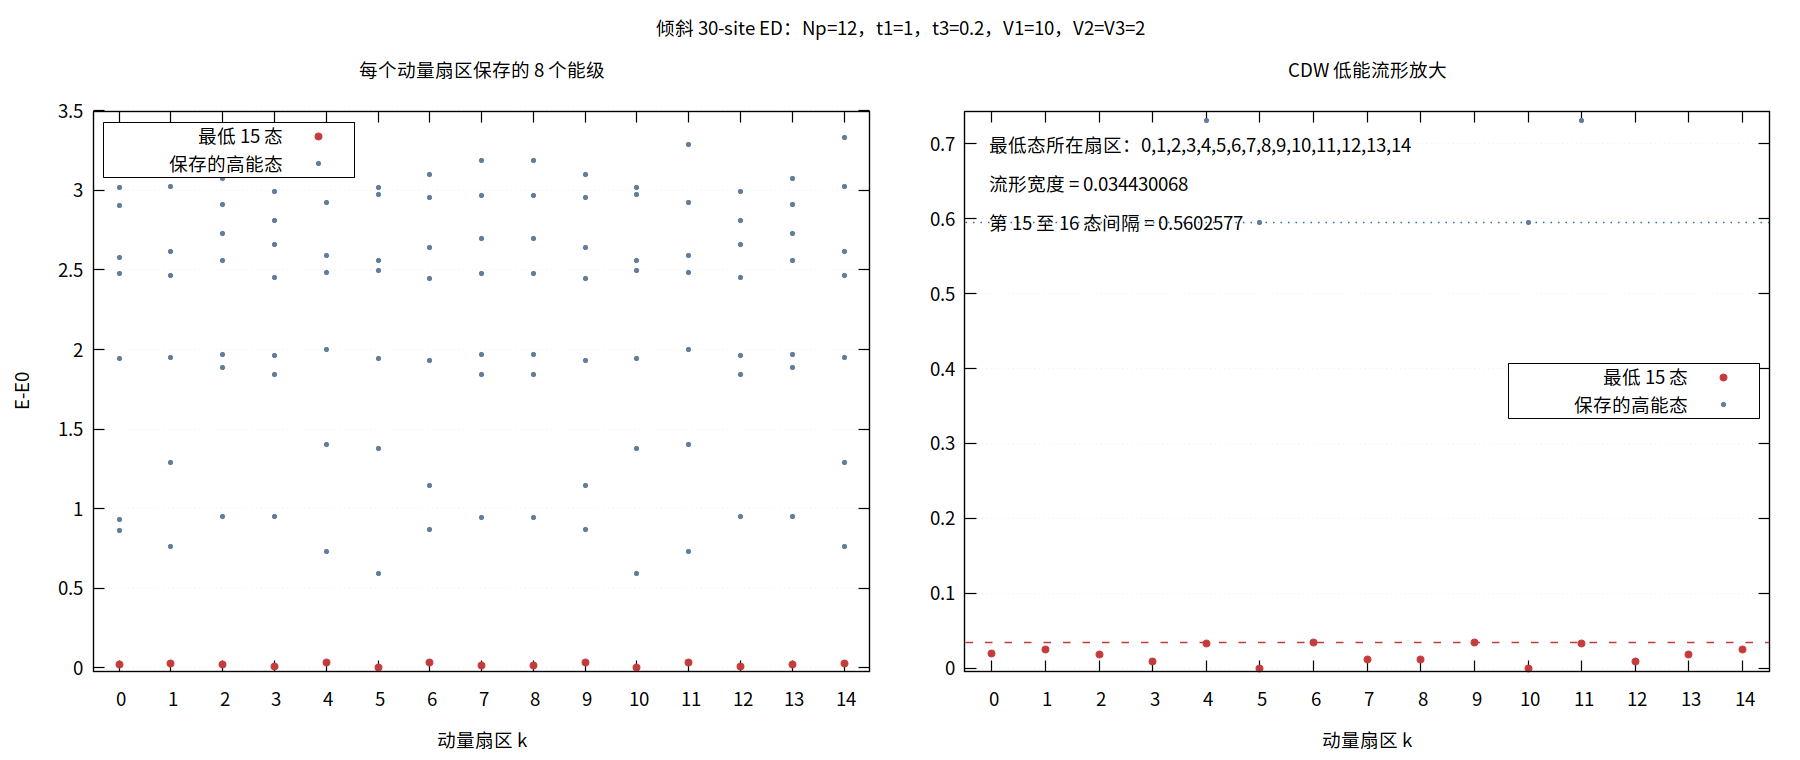
\includegraphics[width=0.96\linewidth]{figures/optical_response/phc30_moderate_manybody_spectrum.png}
\caption{温和参数点的 30-site 多体 ED 能谱。左图给出 15 个动量 sector 中各自
最低 8 个能级；右图放大 CDW 低能流形。红点是最低 15 态，蓝灰点是其余保存的
能级；两条水平线分别标出流形宽度与第 16 态的位置。}
\label{fig:phc30-moderate-spectrum}
\end{figure}

保存态的最大本征方程残差为 \(6.55\times10^{-13}\)，15 个波函数的范数均为 1，
粒子数检验均为 12。大型 \texttt{JLD2} 波函数保存在 W003：
\begin{center}
\small\path{/home/public/shajy/codex_runs/phc30_np12_v1_10_v2_2_v3_2_fqahc/spectrum}.
\end{center}
其中目录名末尾的 \texttt{fqahc} 是计算开始时留下的历史存储标识，不代表本节最终的
相分类。
Git 结果包不复制这些大型文件，只保存每个远端文件的路径、大小和 SHA256，以及
能谱、结构因子和光电导的小型文本数据，因此后续计算可以追溯到同一批波函数。

对每个 sector 的最低态计算静态结构因子，再作 15 态等权平均。平均曲线在
\(q=5,10\) 有两个等高主峰：
\[
  \overline{N(q=5)}=\overline{N(q=10)}=1.283963145836,
\]
而次高峰为
\[
  \overline{N(q=2)}=\overline{N(q=13)}=0.241793403702.
\]
不同 sector 的 \(q=5,10\) 主峰高度分布在
\[
  0.857196848151\ \text{至}\ 1.754306638659.
\]
这说明对称动量本征态之间存在明显的有限尺寸差别，但流形平均仍稳定显示周期三密度序。

\begin{figure}[H]
\centering
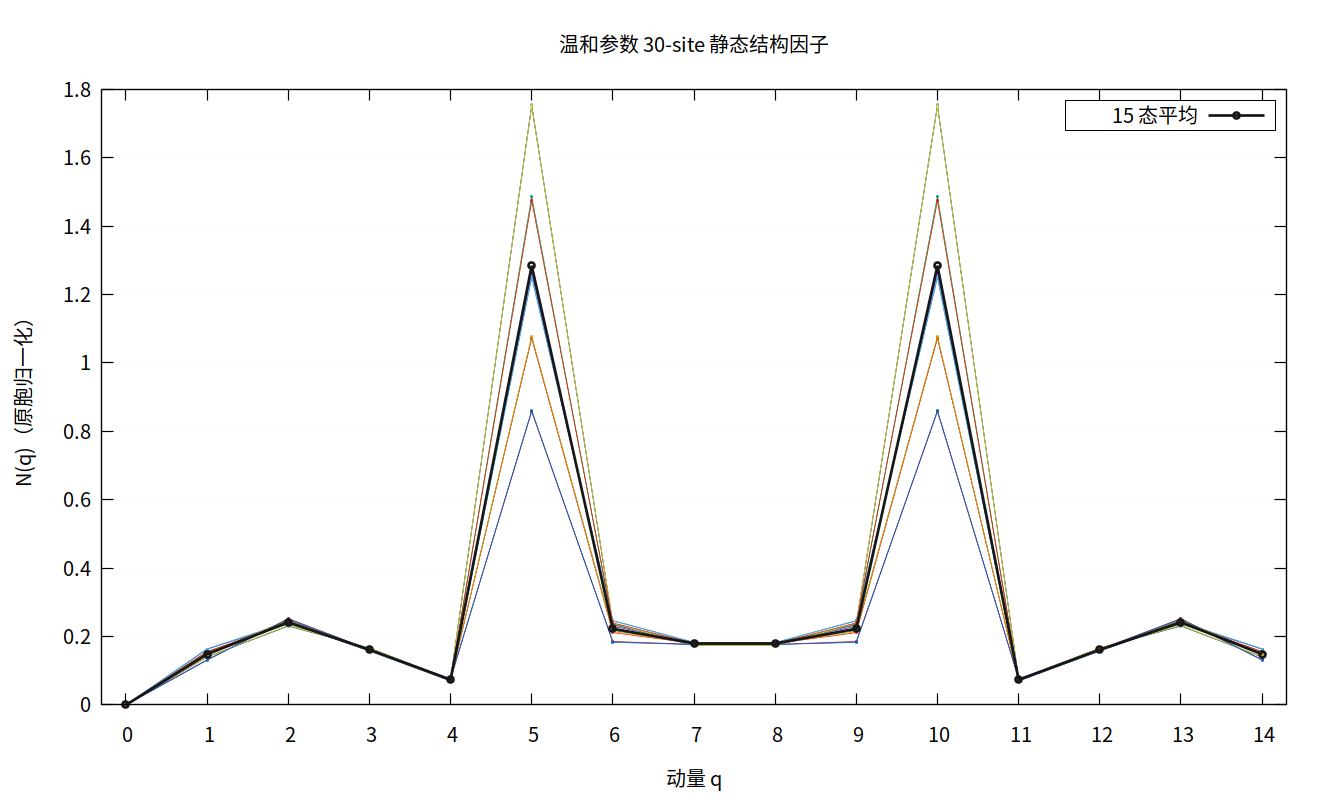
\includegraphics[width=0.82\linewidth]{figures/optical_response/phc30_moderate_structure_factor.png}
\caption{温和参数 CDW 低能流形中 15 态的静态结构因子。彩色细线是各 sector 的最低态，
黑色粗线是 15 态等权平均；\(q=5,10\) 的双峰给出周期三晶体序。纵轴采用
原胞归一化 \(1/N_{\mathrm{uc}}\)。}
\label{fig:phc30-moderate-structure-factor}
\end{figure}

这 15 个 sector 的最低态随后分别作为 response-Lanczos 的起点。响应参数为
\[
  \eta=0.065,\qquad \omega=0:0.002:10,\qquad M=600.
\]
每次计算都从 \(QJ_x|g_k\rangle\) 出发，在同一动量 sector 的 Krylov 空间中求
Kubo resolvent；不显式求出该 sector 的全部激发态。最终对 15 条复电导曲线作
15 态等权平均，并用灰带表示逐频率的 sector 最小值到最大值。这里的 Lanczos
只是大 Hilbert 空间中的 ED 响应算法，\textbf{不是 DMRG 动力学计算}。

\clearpage
\begin{figure}[H]
\centering
\begin{subfigure}{0.48\linewidth}
  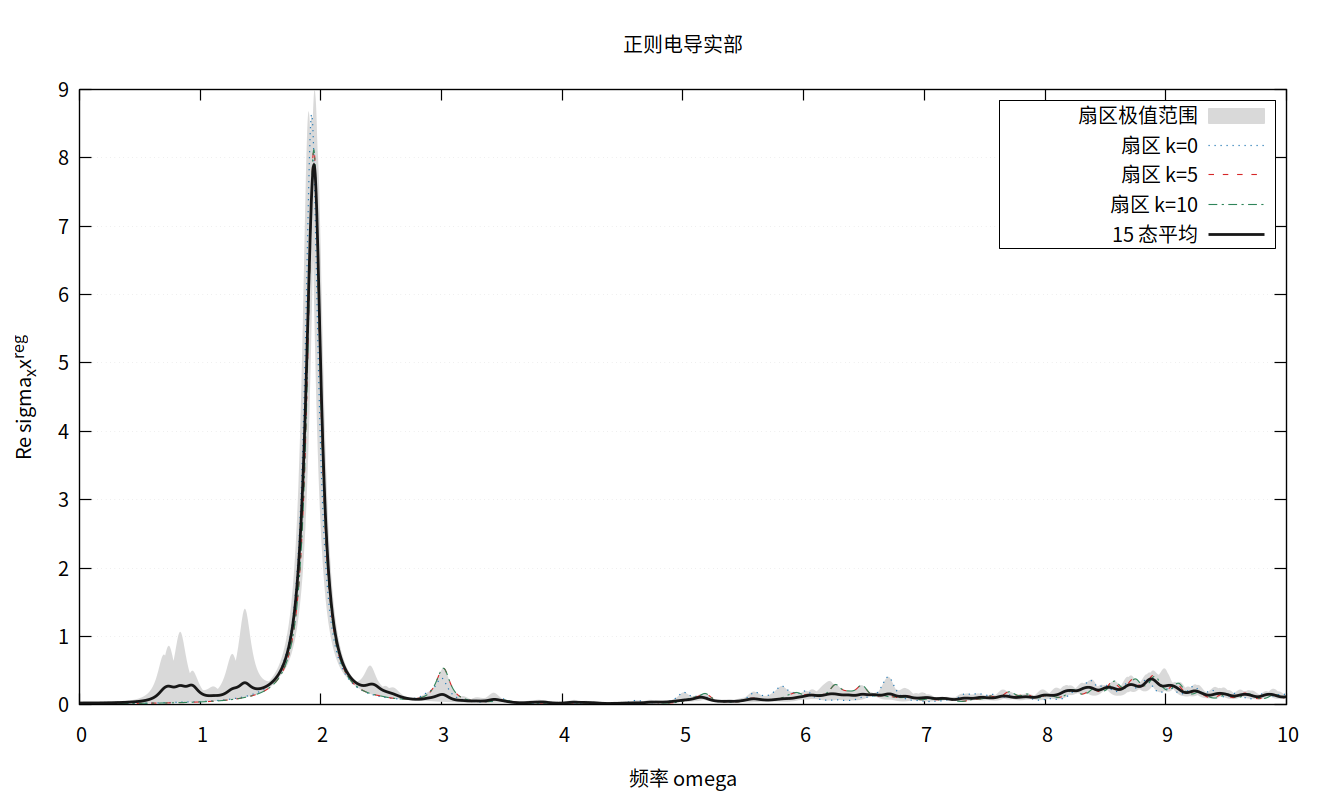
\includegraphics[width=\linewidth]{figures/optical_response/phc30_moderate_sigma_xx_regular_real.png}
  \caption{\(\operatorname{Re}\sigma_{xx}^{\mathrm{reg}}\).}
\end{subfigure}\hfill
\begin{subfigure}{0.48\linewidth}
  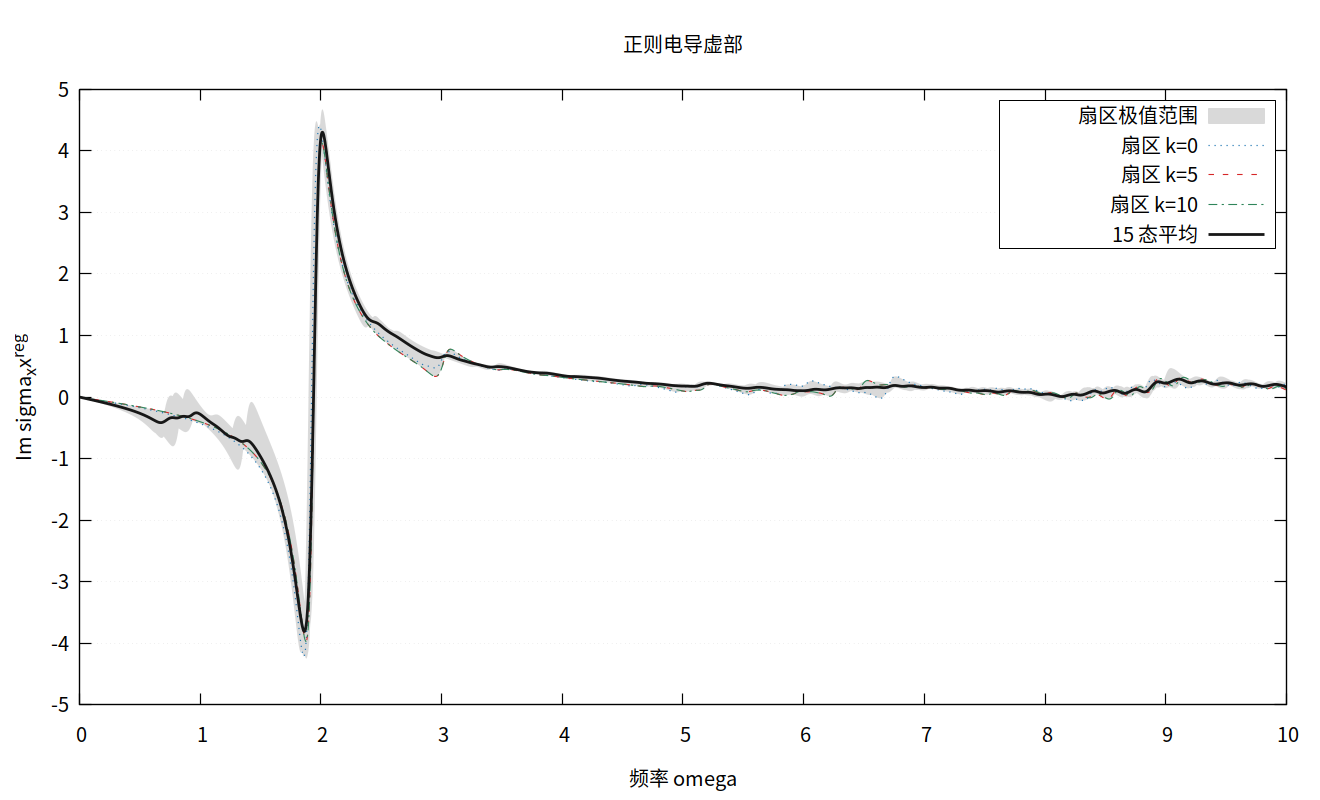
\includegraphics[width=\linewidth]{figures/optical_response/phc30_moderate_sigma_xx_regular_imag.png}
  \caption{\(\operatorname{Im}\sigma_{xx}^{\mathrm{reg}}\).}
\end{subfigure}
\par\medskip
\begin{subfigure}{0.48\linewidth}
  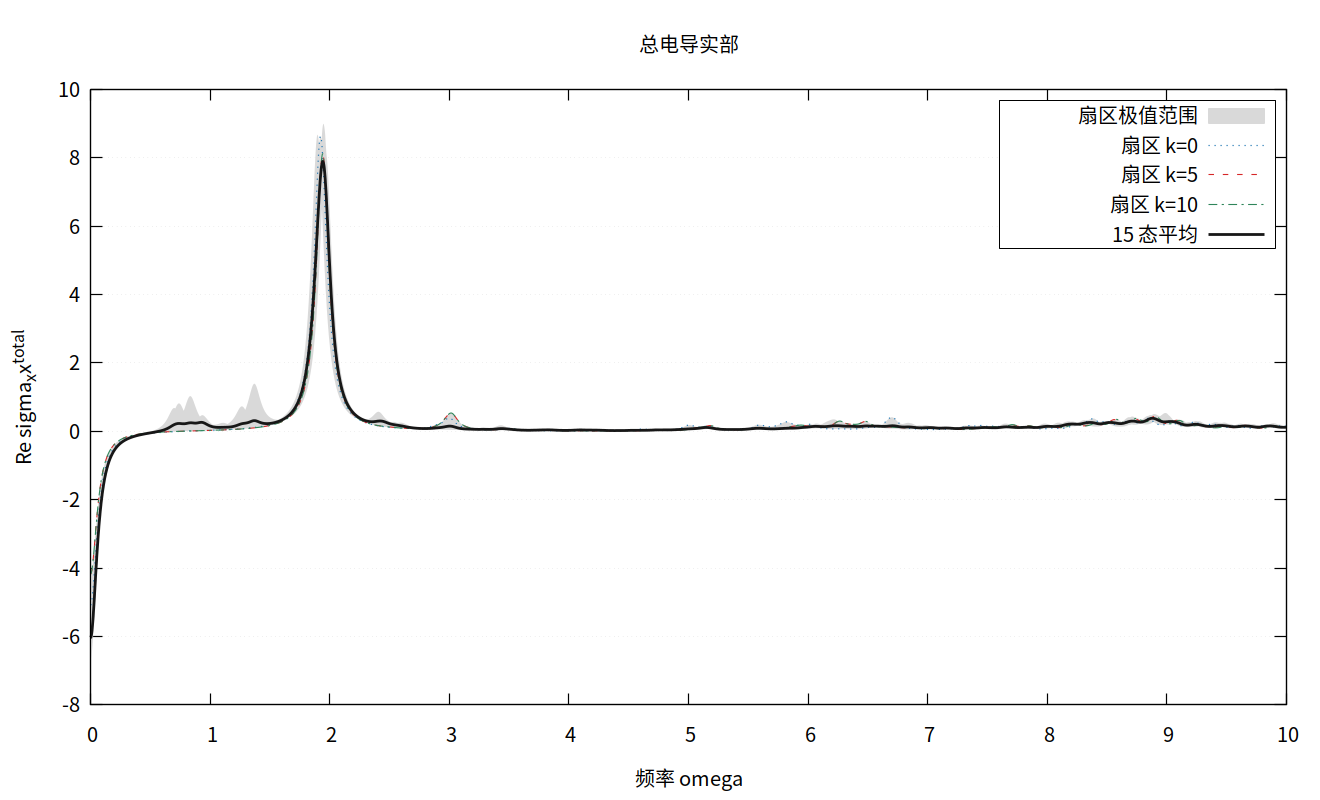
\includegraphics[width=\linewidth]{figures/optical_response/phc30_moderate_sigma_xx_total_real.png}
  \caption{\(\operatorname{Re}\sigma_{xx}^{\mathrm{total}}\).}
\end{subfigure}\hfill
\begin{subfigure}{0.48\linewidth}
  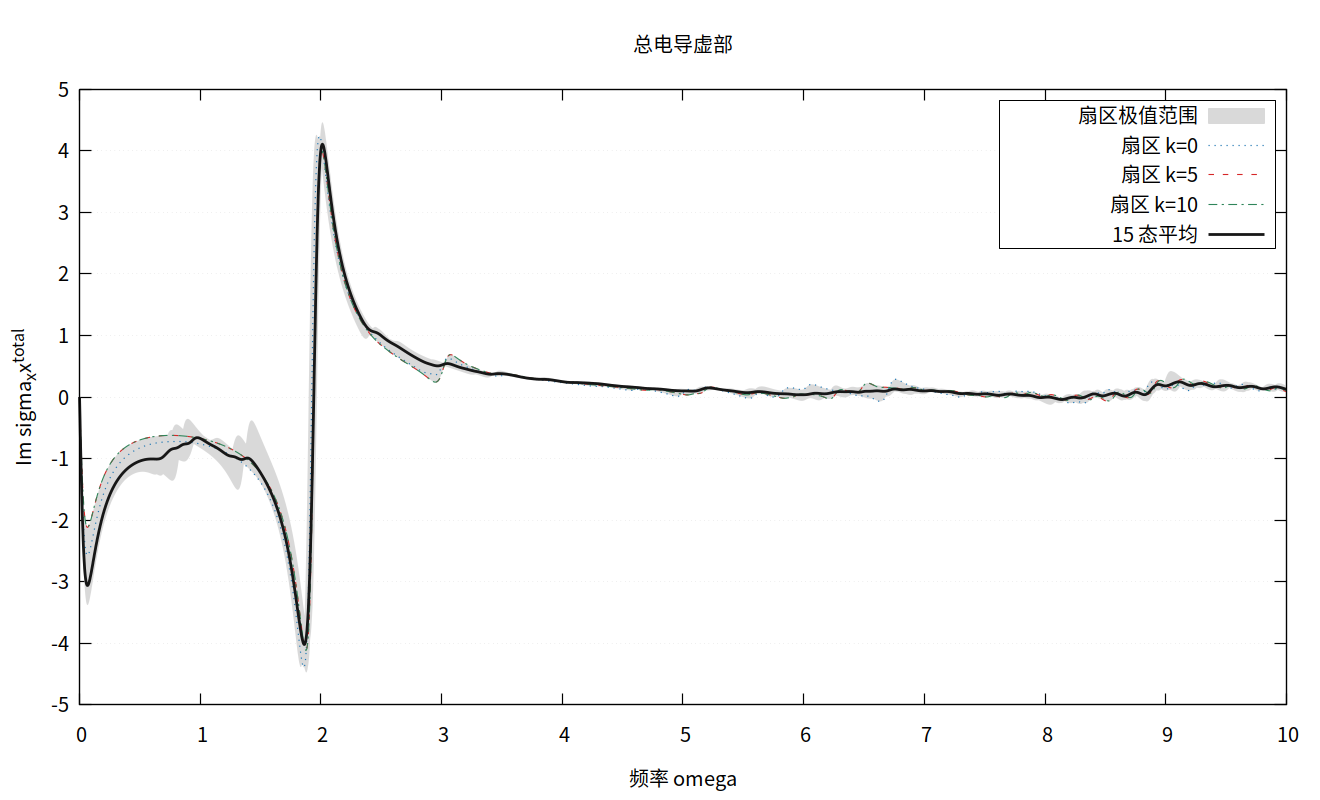
\includegraphics[width=\linewidth]{figures/optical_response/phc30_moderate_sigma_xx_total_imag.png}
  \caption{\(\operatorname{Im}\sigma_{xx}^{\mathrm{total}}\).}
\end{subfigure}
\caption{温和参数 CDW 低能流形的纵向光电导。每条单-sector 曲线均由
response-Lanczos ED 独立计算；黑线是 15 态等权平均，灰带给出 sector 间离散。
四图使用相同的 \(M=600\)、\(\eta=0.065\) 和频率网格。}
\label{fig:phc30-moderate-optical-response}
\end{figure}

平均后的 regular 实部最强吸收峰为
\[
  \omega=1.942,\qquad
  \operatorname{Re}\overline{\sigma_{xx}^{\mathrm{reg}}}=7.893014375259.
\]
各 sector 在 \(\omega\le4\) 的主峰位置为 \(1.898\)--\(1.968\)，各自峰高为
\(8.11425\)--\(8.99645\)。平均谱还在
\(\omega\simeq0.736,0.926,1.370,2.420\) 保留较弱结构，其峰高依次约为
\(0.2749,0.2909,0.3247,0.3053\)。这些峰只表示均匀电流 \(J_x\) 可耦合的
same-sector 中性激发及其谱权重；它们不是完整 many-body gap，也不包含其他动量
sector 中的 optical-dark 激发。

有限 torus 固定 twist 下得到的 Drude 曲率统计为
\[
  \overline{D_{xx}}=-1.628931597494,\qquad
  \operatorname{std}(D_{xx})=0.220228573694,
\]
取值范围为 \(-1.796920178225\)--\(-1.126565223663\)。这里的负值是有限尺寸、固定
twist 处的能量曲率结果，不能直接解释成热力学极限中的负 Drude weight。四幅图中，
regular 实部是有限频率吸收，regular 虚部是相应的色散响应；total 实部和虚部则在
regular 部分上加入用同一 \(\eta\) 展宽的 Drude 项。黑线、灰带和三条代表线分别是
15 态平均、15 sector 极值范围以及 \(k=0,5,10\) 的单-sector 结果。

对 \(k=10\) 将 continued fraction 从 \(M=600\) 截断到 \(M=500\) 后，
\(\omega\le5\) 区间 regular 电导的缩放最大误差为 \(5.66\times10^{-10}\)，
所以图中低频主峰已经收敛。全 \(0\)--\(10\) 区间的对应误差为
\(1.64\times10^{-2}\)，最大差异位于 \(\omega\simeq9.138\)；因此高频弱细峰只作为
有限 \(M\) 的参考。本节的能谱、结构因子和光电导共同描述温和参数 CDW 及其中
current-active 中性激发，不再将该参数点解释为 FQAHC。

\clearpage
\subsection{可以比较与不能直接比较的内容}

\begin{table}[h]
\centering
\small
\caption{历史光学计算与修正后计算的状态。}
\begin{tabular}{p{0.23\linewidth}p{0.33\linewidth}p{0.33\linewidth}}
\toprule
项目 & 历史 ED 图片 & 修正后的基准 \\
\midrule
电磁算符 & 对旧 folded-bond 构造求导；实际 \(x\) 分量为 \(v_1\) & 在有限 torus
折叠前对 \(H(k+A_x\hat{x})\) 作解析求导 \\
面积 & \(A_{\mathrm{old}}=L_1L_2\) & 物理 supercell 面积 \(A=12\sqrt{3}\) \\
所画响应 & 显式 regular Kubo 表达式；tensor 分量随图片而异 & regular、Drude
和 total 复电导 \\
数值方法 & 保存激发态并作显式逐态求和 & 完整 ED 求和与 response-Lanczos 两种方法 \\
验证状态 & 仅作历史记录；峰位和峰高不是修正后的参考结果 & 算符有限差分、exact
求和与 Lanczos continued fraction 已相互检验 \\
\bottomrule
\end{tabular}
\end{table}

可以对照历史图和修正图中谱结构的大致位置，但在使用修正后算符和物理面积重新计算
历史数据之前，绝对峰高、低频行为和 tensor 标签不能直接作定量比较。

旧 \(4\times6\) FCI、30-site 强耦合 CDW 和温和参数 CDW 的系统尺寸、填充或
相互作用参数并不全部相同，因此不能仅根据主峰由 \(4.107\) 变为强 CDW 的 \(1.524\)，
或变为温和参数点的 \(1.942\)，就判断某个相中的完整多体 gap 更小。三套
\(\sigma_{xx}\) 直接给出的都是各自参数点上 \(q=0\) 的 current-active 中性激发及其
谱权重。旧 FCI 光谱还承担 exact sum-over-states 与 response-Lanczos 的数值基准作用；
两组 30-site 结果则展示大 Hilbert 空间中无需全部激发态的 response-Lanczos ED 计算。

强耦合参数点的结构因子和光电导由同一组三重 CDW 基态得到；温和参数点则由隔离的
15 态流形逐 sector 计算后平均。两点都在 \(q=5,10\) 显示周期三晶体序，但光谱结构
并非简单地只相差一个峰：强 CDW 的主要峰在 \(1.524\) 和 \(2.248\)，温和参数点的
平均主峰在 \(1.942\)，并在 \(0.736,0.926,1.370\) 一带具有较弱、sector-dependent
权重。由于相互作用参数不同，这里只能比较 current-active 谱结构；不能仅凭峰位或
峰数判断拓扑。光电导也不能单独确定 many-body Chern number、分数量子化 Hall 响应、
任意子性质或 phason。这些问题还需要 flux insertion/charge pump、完整低能流形和
尺寸标度联合判断。

\section{待完成检查}

\begin{itemize}
  \item 为 \(L_x=2,3,4\) 和多个通量点补充系统的圆柱 ED 基准表。
  \item 比较相同小系统上圆柱 ED 与 DMRG 的密度分布。
  \item 补充分支跟踪诊断：MPS overlap、纠缠谱流和 sector 标签。
  \item 得到完整三 sector 周期后，将泵浦图扩展至 \(6\pi\)。
  \item 补充三重基态中 \(m=0\) 的光学响应，并进一步计算
  \(\sigma_{yy}\) 与 \(\sigma_{xy}\)，用于检查晶体各向异性和 Hall-active 激发。
\end{itemize}

\end{document}
